% ======================================================================
%  The Riemann Hypothesis via a chain of theta lifts:
%  a human-readable account of the Lean proof
%  Ishaan Dixit, November 2026
%  Compiles with pdfLaTeX on Overleaf (TeX Live full).
% ======================================================================
\documentclass[11pt]{article}

\usepackage[utf8]{inputenc}
\IfFileExists{ot2enc.def}{\usepackage[OT2,T1]{fontenc}}{\usepackage[T1]{fontenc}}
\usepackage{lmodern}
\usepackage[margin=1in]{geometry}
\usepackage{amsmath,amssymb,amsthm,mathtools}
\usepackage{booktabs,longtable,array,tabularx}
\usepackage{enumitem}
\usepackage{xcolor}
\usepackage{tikz}
\usetikzlibrary{arrows.meta,positioning}
\usetikzlibrary{decorations.pathreplacing,calc,patterns,shapes.geometric,fit,backgrounds}
\usepackage{pgfplots}
\pgfplotsset{compat=1.18}
\usepgfplotslibrary{fillbetween}
\usepackage{caption}
\captionsetup{font=small,labelfont=bf}
\tikzset{
  fbox/.style={draw, rounded corners=3pt, align=center, font=\small, inner sep=5pt},
  farr/.style={-{Stealth[length=2.2mm]}, thick, gray!70!black},
  hl/.style={draw=blue!70!black, very thick, fill=blue!6},
}

\usepackage[hidelinks]{hyperref}
\usepackage{url}
\setlength{\emergencystretch}{3em}

% ---------- Tate--Shafarevich symbol ----------------------------------
\IfFileExists{ot2enc.def}{%
  \DeclareSymbolFont{cyrletters}{OT2}{wncyr}{m}{n}%
  \DeclareMathSymbol{\Sha}{\mathalpha}{cyrletters}{"58}%
}{\newcommand{\Sha}{\mathrm{Sha}}}

% ---------- Lean names: breakable, underscores allowed ----------------
\urlstyle{tt}
\setlength{\emergencystretch}{3em}
\DeclareUrlCommand\lean{\urlstyle{tt}}

% ---------- evidence labels -------------------------------------------
\definecolor{exactc}{RGB}{0,90,160}
\definecolor{verc}{RGB}{0,120,60}
\definecolor{readc}{RGB}{150,90,0}
\definecolor{oursc}{RGB}{150,0,90}
\newcommand{\Exact}{\textcolor{exactc}{\textsf{\small[Exact]}}}
\newcommand{\Verified}{\textcolor{verc}{\textsf{\small[Verified]}}}
\newcommand{\Reading}{\textcolor{readc}{\textsf{\small[Reading]}}}
\newcommand{\Ours}{\textcolor{oursc}{\textsf{\small[Ours]}}}

% ---------- math macros -----------------------------------------------
\newcommand{\eps}{\varepsilon}
\newcommand{\CC}{\mathbb{C}}
\newcommand{\R}{\mathbb{R}}
\newcommand{\Q}{\mathbb{Q}}
\newcommand{\Z}{\mathbb{Z}}
\newcommand{\N}{\mathbb{N}}
\newcommand{\Oc}{\mathcal{O}}
\newcommand{\re}{\operatorname{Re}}
\newcommand{\len}{\operatorname{len}}
\newcommand{\rk}{\operatorname{rk}}
\newcommand{\Cl}{\operatorname{Cl}}
\newcommand{\ASK}{\mathrm{ASK}}
\newcommand{\MAIN}{\mathrm{MAIN}}
\newcommand{\Err}{\mathrm{Err}}
\newcommand{\Gz}{G_\zeta}
\newcommand{\Gsig}{G_{\mathrm{sig}}}

\theoremstyle{plain}
\newtheorem{theorem}{Theorem}[section]
\newtheorem{proposition}[theorem]{Proposition}
\newtheorem{lemma}[theorem]{Lemma}
\newtheorem{corollary}[theorem]{Corollary}
\theoremstyle{definition}
\newtheorem{definition}[theorem]{Definition}
\newtheorem{remark}[theorem]{Remark}
\newtheorem{question}{Question}

\newenvironment{sketch}{\begin{proof}[Proof sketch (from the Lean proof)]}{\end{proof}}

\setlist{itemsep=2pt,topsep=4pt}

\title{The Riemann Hypothesis via a chain of theta lifts:\\
a human-readable account of the Lean proof}
\author{Ishaan Dixit}
\date{23 November 2026 (v1.1)}

\begin{document}
\maketitle

\begin{abstract}
On 20 November 2026 Levent Alp\"oge released a Lean~4~\cite{lean4} development whose top theorem is
\lean{riemannHypothesis : RiemannHypothesis}, stated with Mathlib's definition. We rebuilt it
independently (175{,}187 modules, 401 minutes on 94 cores): the build is clean and the only axioms
used are \lean{propext}, \lean{Quot.sound} and \lean{Classical.choice}. Apart from a short outline~\cite{alpoge-remark},
no human-readable proof accompanies the release. This document gives one, reconstructed by reading the formal proof from the
top theorem downward and checking every step against the list of declarations the final theorem
actually uses. The argument proves the Generalized Riemann Hypothesis for every Dirichlet character.
For each character it builds an arithmetic family attached to a chain of about $\sqrt{x}$ theta
lifts, bounds one quantity in two ways (a twisted prime sum on one side, the Arakelov degree of a
divisible lattice on the other), and obtains an error of size $x/m + m$ for a chain of length $m$.
Taking $m\approx\sqrt{x}$ gives a square-root bound on a weighted prime sum over windows $[Y,Y^{3/2}]$,
and a windowed form of Landau's theorem turns that into the absence of zeros with
$\re s > 1/2+\eps$. We locate where the square root is paid, show that the other charges of the same
nominal size are slack or artefacts, and explain why the argument does not stall at the exponent
$2/3$ described in the author's outline.
\end{abstract}

\tableofcontents
\newpage

% ======================================================================
\section{Introduction}
% ======================================================================

\subsection{What is proved}

\begin{theorem}[Main theorem, \lean{UpperTheory.EveryCharacter}]\label{thm:main}
For every modulus $N\ge 1$, every Dirichlet character $\chi \bmod N$ and every $s\in\CC$ with
$\re s > 1/2$, if $\chi\neq 1$ or $s\neq 1$ then $L(s,\chi)\neq 0$.
\end{theorem}

The Riemann Hypothesis is the trivial-character case. In the Lean source:
\begin{gather*}
\texttt{riemannHypothesis} := \texttt{rhOfAll},\qquad
\texttt{rhOfAll} := \texttt{rh\_of\_every allChi},\\
\texttt{allChi} := \texttt{FinalTheorems.everyCharacter}.
\end{gather*}
\Exact{} (files \lean{Main.lean}, \lean{MainTheorems.lean} and \lean{MainConclusion.lean}).

\subsection{What this document is, and is not}

This is an account of the \emph{formal} proof. Every statement below is either a paraphrase of a Lean
statement, a summary of a Lean proof, or our interpretation, and we say which. It is not an
independent proof: we have not re-derived the classical inputs (Ferrero--Washington~\cite{ferrero-washington},
Poitou--Tate duality~\cite{nsw}, CM theory~\cite{shimura} and others), which are proved inside the development and checked by the Lean
kernel, and some proofs are summarised rather than reproduced line by line. Where we have not traced
something, we say so (Section~\ref{sec:open}).

\paragraph{Evidence labels.}
\begin{itemize}
\item \Exact: checked against the list of declarations the final theorem uses
  (\texttt{used\_decls.txt}, extracted from the published kernel export: 1{,}468{,}419 declarations
  plus 16{,}314 constructors and recursors).
\item \Verified: read directly in the source (archive sha256 \texttt{9631b4f0\ldots c7fc}).
\item \Reading: interpretation; a specialist should confirm it.
\item \Ours: a finding from our trace that we have not seen posted elsewhere as of 20 November 2026.
\end{itemize}

\subsection{The idea in one paragraph}

Fix a character $\chi$ and a large $x$. The proof attaches to $\chi$, and to two auxiliary primes
$q\equiv 3 \pmod 8$, $d\equiv 7\pmod{16}$, a family of arithmetic objects: Hermitian lattices
indexed by \emph{words} $u$, carried along a chain of $m$ theta lifts between unitary groups whose
signature moves from $(k-1,m)$ to $(k+m-1,0)$, one step per lift. One quantity, $\ASK$, is computed
twice. At the finite places it is a sum over primes of Legendre-type counts weighted by $\chi$; at
the infinite places it is controlled by Chowla--Selberg periods, giving a main term $\MAIN$. A slope
inequality for one common lattice joins the two and yields $\ASK\le \MAIN + \Err$, with
$\Err/(\text{main}) \approx x/m + m$. With $m\approx\sqrt{x}$ this gives a bound of size
$x^{1/2+O(\eps)}$ for a weighted prime sum. Fourier analysis on a small group isolates the prime sum
of $\chi$, and a windowed Landau theorem converts the one-sided bound into zero-freeness.

The author's outline~\cite{alpoge-remark} describes the chain of lifts as playing the role of
multiplicity in Stepanov's method~\cite{iwaniec-kowalski}, and says that charging the lifts one by one would stop at exponent $2/3$. Section~\ref{sec:23}
reconstructs that $2/3$ from the code's own quantities and shows how the code avoids it.

\subsection{Structure of the proof}

\begin{figure}[ht]
\centering
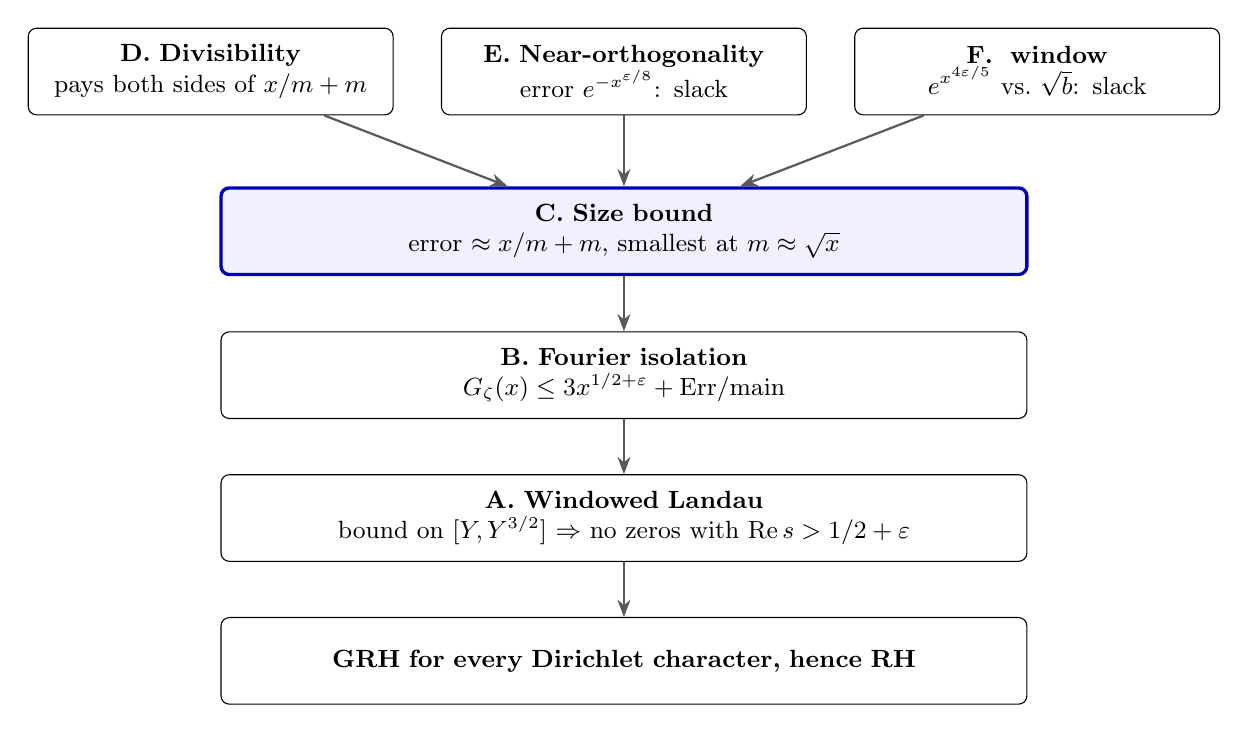
\begin{tikzpicture}[
  box/.style={draw, rounded corners=3pt, align=center, minimum height=11mm, text width=44mm, font=\small},
  wbox/.style={draw, rounded corners=3pt, align=center, minimum height=11mm, text width=100mm, font=\small},
  key/.style={wbox, draw=blue!70!black, very thick, fill=blue!6},
  arr/.style={-{Stealth[length=2.2mm]}, thick, gray!70!black}]
\node[box] (D) {\textbf{D. Divisibility}\\ \mbox{pays both sides of $x/m+m$}};
\node[box, right=6mm of D] (E) {\textbf{E. Near-orthogonality}\\ \mbox{error $e^{-x^{\eps/8}}$: slack}};
\node[box, right=6mm of E] (F) {\textbf{F. $\Sha$ window}\\ \mbox{$e^{x^{4\eps/5}}$ vs.\ $\sqrt b$: slack}};
\node[key, below=9mm of E] (C) {\textbf{C. Size bound}\\ \mbox{error $\approx x/m+m$, smallest at $m\approx\sqrt{x}$}};
\node[wbox, below=7mm of C] (B) {\textbf{B. Fourier isolation}\\ \mbox{$\Gz(x)\le 3x^{1/2+\eps}+\Err/\text{main}$}};
\node[wbox, below=7mm of B] (A) {\textbf{A. Windowed Landau}\\ \mbox{bound on $[Y,Y^{3/2}]$ $\Rightarrow$ no zeros with $\re s>1/2+\eps$}};
\node[wbox, below=7mm of A] (T) {\textbf{GRH for every Dirichlet character, hence RH}};
\draw[arr] (D) -- (C); \draw[arr] (E) -- (C); \draw[arr] (F) -- (C);
\draw[arr] (C) -- (B); \draw[arr] (B) -- (A); \draw[arr] (A) -- (T);
\end{tikzpicture}
\caption{The six steps. The square root is paid once, in the balance of step C, by the divisibility
error of step D. Steps E and F have room to spare.}\label{fig:steps}
\end{figure}

\begin{enumerate}[label=\textbf{\Alph*.}]
\item \textbf{Windowed Landau} (Section~\ref{sec:A}). A one-sided bound on windows $[Y,Y^{1+\delta}]$
  rules out zeros.
\item \textbf{Fourier isolation} (Section~\ref{sec:B}). Averaging over a thick set isolates the
  prime sum of the target character; the auxiliary characters are made harmless by choosing $q,d$
  with a zero-density estimate.
\item \textbf{The size bound} (Section~\ref{sec:C}). The error relative to the main term is about
  $x/m+m$.
\item \textbf{The divisibility layer} (Section~\ref{sec:D}). The degree identity, the common
  lattice, the rank bound and local divisibility.
\item \textbf{Near-orthogonality} (Section~\ref{sec:E}). The words are orthogonal up to
  $\exp(-x^{\eps/8})$.
\item \textbf{The $\Sha$ window} (Section~\ref{sec:F}). Tate--Shafarevich losses over cyclotomic
  layers of degree about $x^2$, resting on formal Iwasawa theory.
\end{enumerate}

% ======================================================================
\section{Notation and parameters}\label{sec:notation}
% ======================================================================

Throughout, $\eps\in(0,1/52)$ is fixed and $x$ is large.

\begin{center}
\small
\renewcommand{\arraystretch}{1.15}
\begin{tabularx}{\textwidth}{@{}l>{\raggedright\arraybackslash}p{62mm}>{\raggedright\arraybackslash}X@{}}
\toprule
Symbol & Value or window & Meaning \\
\midrule
$b$ & $\exp(x^{\eps})$ & common weight; every polynomial loss is negligible against it \\
$a$ & $x\cdot b$ & top weights (\lean{Scale.a}) \\
$\delta_1$ & $x^{-\eps/8}$ & \\
$m$ & $\sqrt{x\delta_1}\le m\le 2\sqrt{x\delta_1}$, even & number of lifts; $m\approx x^{1/2-\eps/16}$ \\
$n=|H|$ & $x^{2+8\eps}\le n\le 2x^{2+8\eps}$ & order of the character group of the host \\
$f$ & $2n$ & number of archimedean places (CM degree) \\
$k$ & $x^{9/2+10\eps}\le k\le 2x^{9/2+10\eps}$, even & second size parameter; word length \\
$t$ & odd, $3m<t$, $t\ge x^{377}$ & size of the cyclotomic twist block \\
$r$ & $k+m-1$ & starting rank \\
$B_0$ & $f\cdot m\cdot b\cdot x^{\eps}$ & per-lift budget (\lean{sizeBudget}) \\
$n_T,\ n_{T2}$ & $n_T\ge x^{-\eps/8}n/2$, $n_{T2}/n\ge x^{-\eps}$ & numbers of top and thick points \\
$\eta=\eta_{Sz}$ & $\le b/(t^3 f k^3)$ & spread of the weights across lifts \\
\bottomrule
\end{tabularx}
\end{center}

\Exact{} The windows for $m,n,k$ are the literal content of \lean{RankVal}
(\lean{.../GlobalTwisting/PairRowIffQdRows.lean:28}); $m$ and $k$ are picked as even numbers in their
windows by \lean{exists_ranks_rankVal_frame}. Concretely \lean{exists_even_between} takes
$m=2\lceil\tfrac12\sqrt{x\delta_1}\rceil=2\lceil\tfrac12x^{1/2-\eps/16}\rceil$, so for fixed $\eps>0$ the chain is
slightly shorter than $\sqrt x$ ($m/\sqrt x\to0$); this was pointed out by hhh2210 in the community
repository's issue~\#5. $B_0$ is a definition, not an estimate:
\lean{SizeData_2.B0 := sizeBudget D.R x eps}, and the hypothesis \lean{BNBounds} is proved by
equality ($B_0 = 2|H|\cdot m\cdot b\cdot x^\eps$).

\begin{figure}[ht]
\centering
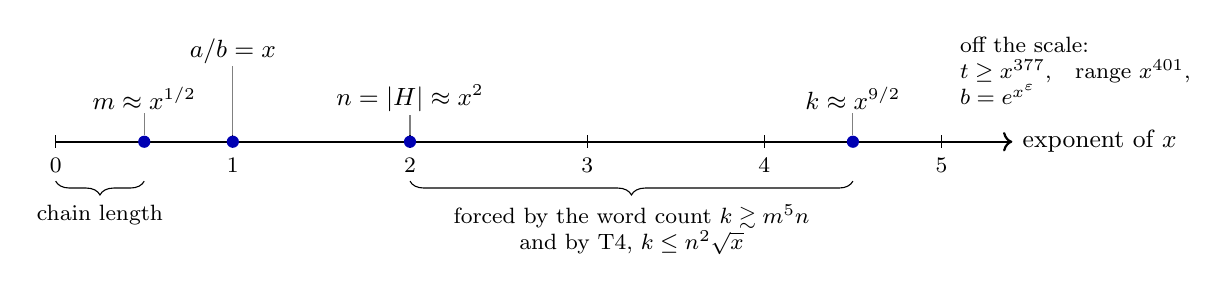
\begin{tikzpicture}[x=2.25cm]
\draw[->, thick] (0,0) -- (5.4,0) node[right, font=\small] {exponent of $x$};
\foreach \v in {0,1,2,3,4,5} \draw (\v,0.08) -- (\v,-0.08) node[below, font=\footnotesize] {$\v$};
\foreach \v/\lab/\h in {0.5/{$m\approx x^{1/2}$}/0.55, 1/{$a/b = x$}/1.15, 2/{$n=|H|\approx x^{2}$}/0.55, 4.5/{$k\approx x^{9/2}$}/0.55}
  { \fill[blue!70!black] (\v,0) circle (2.2pt); \draw[gray] (\v,0.08) -- (\v,\h-0.12); \node[font=\small, fill=white, inner sep=1pt] at (\v,\h) {\lab}; }
\draw[decorate, decoration={brace, amplitude=5pt, mirror}] (0,-0.5) -- (0.5,-0.5) node[midway, below=5pt, font=\footnotesize] {chain length};
\draw[decorate, decoration={brace, amplitude=5pt, mirror}] (2,-0.5) -- (4.5,-0.5) node[midway, below=5pt, font=\footnotesize, align=center] {forced by the word count $k\gtrsim m^5 n$\\ and by T4, $k\le n^2\sqrt x$};
\node[font=\footnotesize, align=left, anchor=west] at (5.05,0.9) {off the scale:\\ $t\ge x^{377}$,\ \ $\Sha$ range $x^{401}$,\\ $b=e^{x^\eps}$};
\end{tikzpicture}
\caption{The sizes of the family as powers of $x$ (up to $x^{O(\eps)}$). Only $m\approx\sqrt x$ is
chosen; the exponents $2$ and $9/2$ of $n$ and $k$ follow from it (Section~\ref{sec:windows}). The
weight $b=\exp(x^\eps)$ is larger than every power of $x$, so every polynomial loss is negligible
against it.}\label{fig:ladder}
\end{figure}



\paragraph{Ranks and signatures.} \Verified{} (\lean{Formalism/LocalRingCardinality/Params.lean})
\[
N(j) = k + j(t+1),\qquad \operatorname{rankY}(j) = r + jt,\qquad
\operatorname{sig}(j) = (k+j-1,\ m-j),\qquad j=0,\dots,m.
\]
So the chain starts at signature $(k-1,m)$ and ends at the definite signature $(k+m-1,0)$; each
lift moves one unit across and adds $t+1$ rows.

\begin{figure}[ht]
\centering
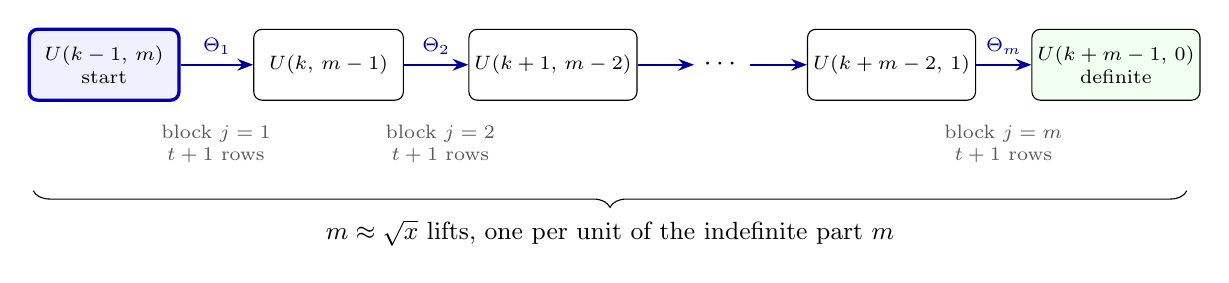
\begin{tikzpicture}[
  sig/.style={draw, rounded corners=3pt, minimum width=19mm, minimum height=9mm, font=\scriptsize, align=center, inner sep=2pt},
  lift/.style={-{Stealth[length=2mm]}, thick, blue!60!black}]
\node[sig, hl] (s0) at (0,0) {$U(k-1,\,m)$\\ start};
\node[sig] (s1) at (2.85,0) {$U(k,\,m-1)$};
\node[sig] (s2) at (5.7,0) {$U(k+1,\,m-2)$};
\node (dots) at (7.85,0) {$\cdots$};
\node[sig] (s3) at (10.0,0) {$U(k+m-2,\,1)$};
\node[sig, fill=green!6] (s4) at (12.85,0) {$U(k+m-1,\,0)$\\ definite};
\draw[lift] (s0) -- node[above, font=\scriptsize] {$\Theta_1$} (s1);
\draw[lift] (s1) -- node[above, font=\scriptsize] {$\Theta_2$} (s2);
\draw[lift] (s2) -- (dots);
\draw[lift] (dots) -- (s3);
\draw[lift] (s3) -- node[above, font=\scriptsize] {$\Theta_m$} (s4);
\foreach \i/\x in {1/1.42,2/4.27,m/11.42}
  \node[font=\scriptsize, gray!70!black, align=center] at (\x,-1.0) {block $j=\i$\\ $t+1$ rows};
\draw[decorate, decoration={brace, amplitude=6pt, mirror}] (-0.9,-1.6) -- (13.75,-1.6)
  node[midway, below=7pt, font=\small] {$m\approx\sqrt x$ lifts, one per unit of the indefinite part $m$};
\end{tikzpicture}
\caption{The chain of theta lifts. Each lift moves the signature one step towards the definite
group and adjoins one block of $t+1$ rows. The indefinite part $m$ of the start is both the number of
lifts and, in Section~\ref{sec:D}, the Bloch--Kato rank of every piece.}\label{fig:chain}
\end{figure}



% ======================================================================
\section{Step A: from a bound on windows to the absence of zeros}\label{sec:A}
% ======================================================================

\subsection{The quantity bounded}

\begin{definition}[\lean{Deduction.Gchi}, \lean{Formalism.Gz}]
For $y\ge 1$ let $\operatorname{ramp}_\chi(y)=\sum_{n\le y}\Lambda(n)\chi(n)\,(y/n-1)$. Put
\[
G_\chi(y) =
\begin{cases}
\operatorname{ramp}_\chi(y) - y\log y + (1+\gamma)y, & \chi = 1,\\[2pt]
\operatorname{ramp}_\chi(y) + y\,\dfrac{L'(1,\chi)}{L(1,\chi)}, & \chi\neq 1.
\end{cases}
\]
For $\chi=1$ this is $\Gz(x) = \sum_{n\le x}\Lambda(n)(x/n-1) - x\log x + (1+\gamma)x$
(\lean{Formalism/StatementOC.lean:13}).
\end{definition}

$\operatorname{ramp}_\chi(y) = \int_1^y \psi(t,\chi)\,dt/t$ is the logarithmic Riesz mean of the
Chebyshev function, and $G_\chi$ is its remainder after the main term. RH is equivalent to
$\Gz(x) = O(x^{1/2+\eps})$.

\begin{remark}[\Verified]
In one place in the development the von Mangoldt function appears under the name
\lean{abelian_2}, defined as \lean{ArithmeticFunction.vonMangoldt}. Searches for the usual names
miss it; Step~5 of the author's timeline (``definitively switch to $\Lambda$'') is exactly the
expression $\Gz$ above.
\end{remark}

\subsection{The windowed Landau theorem}

\begin{definition}[\lean{CharFamily}]
A character family is a finite set of Dirichlet characters $\chi_i \bmod N_i$ with weights
$a_i>0$, the trivial character occurring only with modulus $1$. Put
$G_m(y) = \sum_i a_i \re G_{\chi_i}(y)$.
\end{definition}

\begin{theorem}[Windowed Landau, \lean{zeroFree_of_rpow_window}, \Exact]\label{thm:landau}
Let $0<\theta<1$, $\delta>0$, $C$ real. Suppose that for every $Y_0$ there is $Y\ge Y_0$ with
\[
G_m(y)\le C\,y^{\theta}\qquad\text{for all } y\in[Y,\,Y^{1+\delta}].
\]
Then $L(s,\chi_i)\neq 0$ for every $i$ and every $\re s>\theta$.
\end{theorem}

\begin{sketch}
The proof goes through \lean{lemmaL} and \lean{landau_window}. \lean{poleData} builds a function
$\Phi$ (the Mellin transform of $G_m$, assembled from the characters and their inverses) whose poles
in $\re s>0$ are exactly the zeros of the $L(s,\chi_i)$ and of their conjugates, and shows the
zeros are isolated and have real part at most $2$ (\lean{landau_pole_re_le}). Suppose a zero
$\rho_0$ has $\re\rho_0>\theta$. \lean{landau_window_key} produces, from the window hypothesis
(in the integrated form \lean{WindowHypU}), a real $\sigma$ and a growth bound for the Mellin
integral restricted to windows. \lean{landau_dichotomy} then splits into two cases: either there is
a zero-free disc around a real point with a zero on its boundary, or there is an isolated real zero
$\beta$ in the region; \lean{landau_nearest} picks the nearest pole. In both cases the window bound
contradicts the growth forced by the pole (\lean{landau_growth_contra},
\lean{landau_window_contra}).
\end{sketch}

\begin{figure}[ht]
\centering
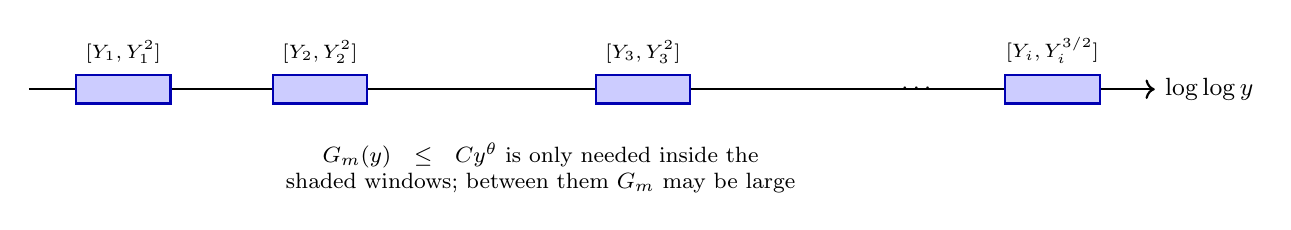
\begin{tikzpicture}[x=1.0cm]
\draw[->, thick] (0,0) -- (14.3,0) node[right, font=\small] {$\log\log y$};
\foreach \a/\lab in {0.6/1, 3.1/2, 7.2/3}{
  \fill[blue!20] (\a,-0.18) rectangle (\a+1.2,0.18);
  \draw[blue!70!black, thick] (\a,-0.18) rectangle (\a+1.2,0.18);
  \node[font=\scriptsize, above] at (\a+0.6,0.2) {$[Y_{\lab},Y_{\lab}^{2}]$};
}
\node[font=\small] at (11.3,0) {$\cdots$};
\fill[blue!20] (12.4,-0.18) rectangle (13.6,0.18); \draw[blue!70!black, thick] (12.4,-0.18) rectangle (13.6,0.18);
\node[font=\scriptsize, above] at (13,0.2) {$[Y_i,Y_i^{3/2}]$};
\node[font=\footnotesize, align=center, text width=8.5cm] at (6.5,-1.0)
  {$G_m(y)\le C y^{\theta}$ is only needed inside the shaded windows; between them $G_m$ may be large};
\end{tikzpicture}
\caption{The hypothesis of the windowed Landau theorem (on a $\log\log$ scale each window $[Y,Y^{3/2}]$
has the same length $\log(3/2)$). A sequence of windows reaching to infinity is enough to rule out zeros
with $\re s>\theta$.}\label{fig:windows}
\end{figure}

\begin{remark}[Why one sign is enough, \Reading{} checked by arithmetic]
In the levels actually used, \lean{Level.cyc psi} is the cyclic group generated by a primitive
$\psi$, each of its $o-1$ nontrivial members weighted $1/(3o+1)$. Every Dirichlet coefficient of the
combined series is then at least $\Lambda(n)\bigl(1-\tfrac{o-1}{3o+1}\bigr)>0$. Positive
coefficients are exactly what Landau's argument needs, so an upper bound on $G_m$ alone forces
zero-freeness. The classical theorem needs the bound for all large $y$; here a sequence of windows
reaching to infinity suffices.
\end{remark}

\begin{remark}[\Verified]
A different Landau theorem, \lean{zero_free_of_Chebyshev_growth} in the namespace
\lean{Formalism.HC.Landau}, is proved in the archive but not used.
\end{remark}

\subsection{The square-root bound and the assembly}

\begin{theorem}[\lean{UpperTheory.Comparison_2.core_gm}, \Exact]\label{thm:coregm}
For every level $\Lambda$ and $\eps>0$ there is $x_1$ such that for all $x\ge x_1$, every frame and
host satisfying the hypotheses \lean{EAtH} and \lean{CoreAtH},
\[
\Lambda.G_m(x)\le x^{1/2+(e_D+e_L+7)\eps}.
\]
\end{theorem}

\lean{CoreAtH} packages the data record of Section~\ref{sec:D} together with the size windows, in
particular \lean{RestSize}: $x^{1/2-\eps}\le m$ and $k\le n^2x^{1/2-\eps}$. The chain from
Theorem~\ref{thm:coregm} to Theorem~\ref{thm:main} is (\Verified):
\lean{formB} $\to$ \lean{zeroFree_of_rpow_window} $\to$ \lean{level_of_tiedWin},
\lean{zeroFreeOn_of_tiedWin_cyc} $\to$ \lean{zeroFreeAll_of_topG} $\to$ \lean{imprimitive}
$\to$ \lean{EveryCharacter}.

\begin{corollary}
Every later step only has to hold for $x$ in windows. \Exact{} The $\Sha$ window of
Section~\ref{sec:F} is stated on $[Y,Y^2]$ with $Y\ge X^{1/J}$, and \lean{supplyChi} turns it into
host fields on windows with exponent $3/2$ (\lean{HostExW}), so the Landau step is applied
with $\delta=1/2$, that is, on windows $[Y,Y^{3/2}]$. We thank Manvir Jaswal, whose
guide~\cite{jaswal} states the windows this way, for the correction.
\end{corollary}

% ======================================================================
\section{Step B: isolating the target character}\label{sec:B}
% ======================================================================

\subsection{The group and its characters}

The host comes with a finite abelian group $H$ and a group $E_0$ with four characters
$0,\psi,\chi,\chi\psi$ (\lean{psC}, \lean{chC}, \lean{chpsC}). \Exact{}
(\lean{CharacterSignsAtBaseClass}) At the base class $g_0$:
\[
\chi(g_0)=-1,\qquad \psi(g_0)=+1,\qquad \chi\psi(g_0)=-1.
\]
Define
\[
\Gsig = G_0 + G_\psi - G_\chi - G_{\chi\psi}.
\]
This is the Fourier projection onto the class of $g_0$; its trivial part $G_0$ carries the prime
sum of the target.

\begin{figure}[ht]
\centering
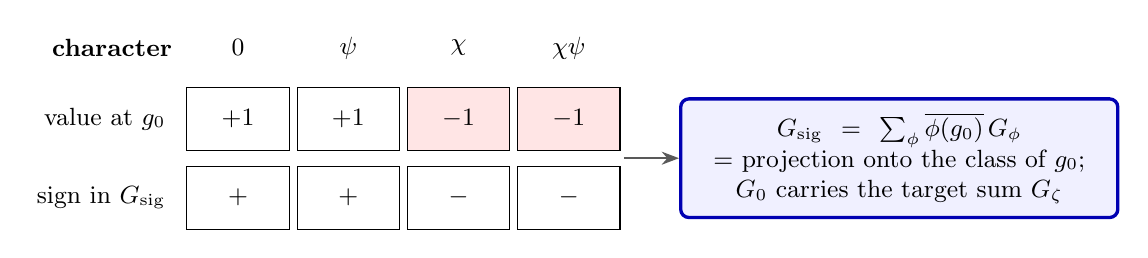
\begin{tikzpicture}[cell/.style={draw, minimum width=13mm, minimum height=8mm, font=\small}]
\node[font=\small\bfseries] at (-1.6,0.9) {character};
\foreach \c/\x in {$0$/0,$\psi$/1.4,$\chi$/2.8,$\chi\psi$/4.2} \node[font=\small] at (\x,0.9) {\c};
\node[font=\small, anchor=east] at (-0.8,0) {value at $g_0$};
\node[cell] at (0,0) {$+1$}; \node[cell] at (1.4,0) {$+1$};
\node[cell, fill=red!10] at (2.8,0) {$-1$}; \node[cell, fill=red!10] at (4.2,0) {$-1$};
\node[font=\small, anchor=east] at (-0.8,-1) {sign in $G_{\mathrm{sig}}$};
\node[cell] at (0,-1) {$+$}; \node[cell] at (1.4,-1) {$+$};
\node[cell] at (2.8,-1) {$-$}; \node[cell] at (4.2,-1) {$-$};
\node[fbox, hl, anchor=west, text width=52mm] (t) at (5.6,-0.5)
  {$\Gsig=\sum_\phi \overline{\phi(g_0)}\,G_\phi$\\ $=$ projection onto the class of $g_0$;\\ $G_0$ carries the target sum $\Gz$};
\draw[farr] (4.9,-0.5) -- (t.west);
\end{tikzpicture}
\caption{Fourier isolation on $E_0$. The signs of $\Gsig$ are the conjugate character values at
the base class, so averaging keeps exactly the class of $g_0$. The three nontrivial terms are
bounded by $x^{1/2+\eps}$ each, because the auxiliary primes were chosen to make them so.}\label{fig:signs}
\end{figure}



\subsection{An exact identity}

\begin{proposition}[\lean{Deduction.ch_balance}, \Exact]\label{prop:chbalance}
For every $a>0$, $t\in H$, weights $w>0$ on the admissible set and $N$ large enough,
\[
\ASK(D,N,a,t,w) - \MAIN(\ell,a,w) = \operatorname{De}(D,\ell,a,t,w),
\]
where $\operatorname{De}$ is an explicit combination of the $G_\psi$ evaluated at $a/w$.
\end{proposition}

This is an identity, not an inequality: it expands the counted quantity $\ASK$ over all characters
of $E_0\times H$ (\lean{askExp}). Averaging over the thick set collapses the character sum.

\begin{proposition}[\lean{ThickPartTranslateMean}, \Exact]
For a thick set $T_2$ of density $\delta_2 = |T_2|/|H|$,
\[
\frac{1}{|H|}\sum_{u_0\in H}\frac{1}{|\Phi|}\sum_{\substack{g\notin\Phi\\ g \text{ thick at } u_0}}
\sum_{\psi}\overline{\psi(g)}\, b\,G_\psi(A/b) \;=\; \frac{\delta_2\, b}{2}\,\Gsig(A/b).
\]
\end{proposition}

\subsection{The growth inequality}

\begin{theorem}[\lean{GrowthInequalityExplicit}, \Exact]\label{thm:growth}
Under \lean{GrowthInequalityHypotheses} (which include $\mathrm{topExcess}\le \Err$ and
\lean{ValuesAtX}),
\[
|T_T|\, m\, b\,\frac{\delta_2}{2}\Bigl(\Gz(x) - 3x^{1/2+\eps} - \mathrm{moveCost}\Bigr)
\le \Err + |T_T|\, m\cdot 2f_{Pl}(x+1)\,b\,\theta + |T_T|\, m\cdot 6f_{Pl}(x+1)(\eta+1),
\]
where $\mathrm{topExcess} = \frac{1}{|H|}\sum_{u_0}\sum_{t\in T_T}\sum_{j}\bigl(\ASK - \re\MAIN\bigr)$
and $\mathrm{moveCost} = C_d + 3(\log(x+1)+C_d+C_L\log x)$.
\end{theorem}

The term $3x^{1/2+\eps}$ comes from \lean{signal_term}: for $|y-x|\le 1$,
\[
\Gz(x) - 3x^{1/2+\eps} - \mathrm{moveCost} \le \re\Gsig(y),
\]
using \lean{ValuesAtX}: $\|G_\psi(x)\|\le x^{1/2+\eps}$ and $\|\ell(\psi)\|\le C_L\log x$ for the
three nontrivial characters of $E_0$, and a Lipschitz bound (\lean{DerivInt}).

\begin{remark}[\Reading]
Dividing Theorem~\ref{thm:growth} by $|T_T|\,m\,b\,\delta_2/2$ gives
\[
\Gz(x)\le 3x^{1/2+\eps} + \frac{\Err}{|T_T|\,m\,b\,\delta_2/2}+\dots
\]
So the whole problem is to prove $\Err\lesssim |T_T|\,m\,b\,x^{1/2+O(\eps)}$. Sections~\ref{sec:C} and~\ref{sec:D} do exactly that.
\end{remark}

\subsection{The auxiliary characters are chosen, not controlled}

The characters $\psi,\chi,\chi\psi$ are twists by the quadratic characters of the auxiliary primes
$q\equiv 3\pmod 8$ and $d\equiv 7\pmod{16}$ (\lean{PrimePair}). Their bounds in \lean{ValuesAtX}
come from the following chain, all \Exact:
\lean{QH.pairEx} $\leftarrow$ \lean{pair_exists} $\leftarrow\cdots\leftarrow$
\lean{count_bad_core} $\leftarrow$ \lean{ZD.zero_density_box}.

\begin{definition}[\lean{Box}]
For a character $\psi$, $\mathrm{Box}(Q,C,\tau,Y,X,\psi)$ means: $\psi$ has a good conductor,
$\|L'/L(1,\psi)\|\le C\log Y$, and $\|G_\psi(y)\|\le y^{1/2+\tau}$ for all $y\in[Y,X]$.
\end{definition}

\begin{theorem}[\lean{count_bad_core}, \Exact]
There is $C\ge 0$ such that for $Q\ge 3$ and any set $S$ of primes $q>F$ each carrying a primitive
character of conductor $fq\le Q$, $f\le F$, without a zero-free box,
$|S|\le C\,Q^{1/4}$.
\end{theorem}

The zero-density estimate \lean{zero_density_box} (compare~\cite[Ch.~10]{iwaniec-kowalski}) is assembled from a coefficient square bound, zero
detection by a mollifier identity, a duality inequality and a pair-twist bound.

\begin{remark}[\Reading]
The auxiliary $L$-functions are not proved to satisfy GRH. The proof picks $q$ and $d$ outside the
few bad moduli. The target character is the only one whose $L$-function is not controlled in
advance.
\end{remark}

\subsection{The thick set}

\begin{theorem}[\lean{hostThickExists}, \Exact]
There is $C>0$ such that for all $n$ and $L\ge 2$ there is $T\subset\N$ with $4Ls<n$ for $s\in T$,
no relation $j(s_2-s_1)=i(s_3-s_1)$ with distinct $s_1,s_2,s_3\in T$, $0<|i|,|j|\le L$, $i\neq j$,
and
\[
|T|\ \ge\ \frac{n\,e^{-C\sqrt{\log n\,\log L}}}{L}.
\]
\end{theorem}

\Reading{} The density $\delta_2$ enters only through the division above and costs $x^{o(1)}$.

% ======================================================================
\section{Step C: the size bound, where $\sqrt{x}$ is paid}\label{sec:C}
% ======================================================================

\subsection{The balance}

\begin{theorem}[\lean{proposition_size_bound}, \Exact]\label{thm:size}
In the abstract setting of \lean{GrowthSizeBound},
\[
n_T\,m\,b\,\frac{\delta_2}{2}\bigl(G(x)-4x^{1/2+\eps}\bigr)\le \Err + \frac{2n_T m b}{x},
\]
\[
\Err \le x^{C\eps}\Bigl[n_T a_E\Bigl(1+\frac{m^2}{k}\Bigr) + m\cdot B_0 + m\cdot\frac{n_{T2}\,k\,b\,x^{\eps}}{n^2x^{-\eps}}\Bigr],
\]
and under the windows below, $G(x)\le x^{1/2+(C+3)\eps}$.
\end{theorem}

Dividing each error term by the size $n_T\,m\,b$ of the main term (lemmas \lean{SZ.T1}--\lean{SZ.T4},
\Verified):

\begin{center}
\renewcommand{\arraystretch}{1.2}
\begin{tabular}{@{}llll@{}}
\toprule
Term & After dividing & Bound & Needs \\
\midrule
$n_T a_E$ & $a_E/(mb)\approx \mathbf{x/m}$ & $\le x^{1/2+\eps}$ & $m\ge \sqrt{x}$ (T1)\\
$n_T a_E m^2/k$ & $xm/k$ & $\le 2$ & $k\ge xm$ (T2)\\
$m\cdot B_0$ & $2nm/n_T\approx \mathbf{m}$ & $\le x^{1/2+\dots}$ & $m\le\sqrt{x}$ (T3)\\
$m\cdot(k\text{-term})$ & $k/(n\,n_T)$ & $\le x^{1/2+\dots}$ & $k\le n^2\sqrt{x}$ (T4)\\
\bottomrule
\end{tabular}
\end{center}

So, relative to the main term, the error is about $x/m+m$, and both pieces are $\sqrt{x}$ exactly
when $m\asymp\sqrt{x}$.

\begin{figure}[ht]
\centering
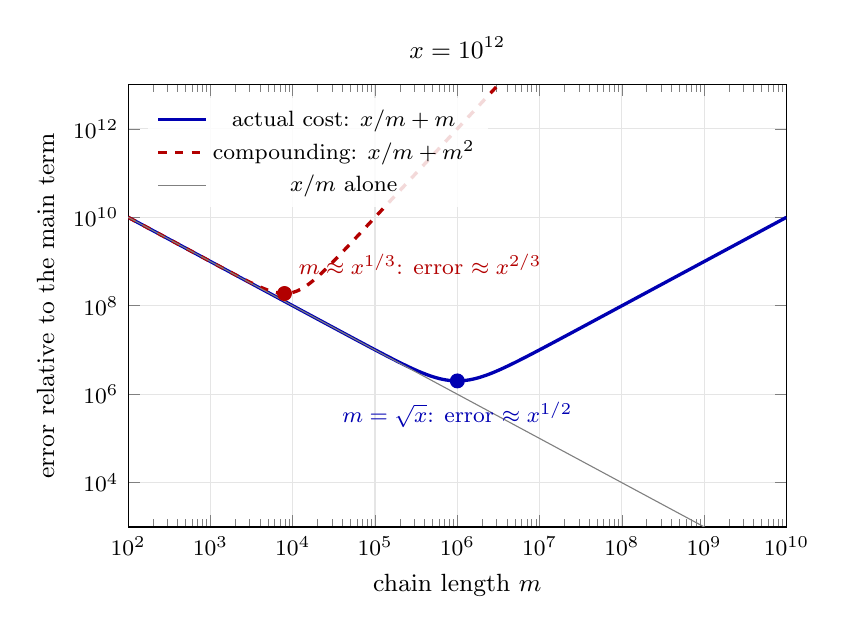
\begin{tikzpicture}
\begin{axis}[
  width=0.82\textwidth, height=7.2cm,
  xmode=log, ymode=log, log basis x=10, log basis y=10,
  xmin=1e2, xmax=1e10, ymin=1e3, ymax=1e13,
  xlabel={chain length $m$}, ylabel={error relative to the main term},
  legend pos=north west, legend style={font=\footnotesize, draw=none, fill=white, fill opacity=0.85, text opacity=1},
  grid=major, grid style={gray!20}, tick label style={font=\footnotesize}, label style={font=\small},
  title={$x=10^{12}$}, title style={font=\small}]
\addplot[domain=1e2:1e10, samples=200, blue!70!black, very thick] {1e12/x + x};
\addlegendentry{actual cost: $x/m+m$}
\addplot[domain=1e2:1e10, samples=200, red!70!black, very thick, dashed] {1e12/x + x^2};
\addlegendentry{compounding: $x/m+m^2$}
\addplot[domain=1e2:1e10, samples=2, gray, thin] {1e12/x};
\addlegendentry{$x/m$ alone}
\addplot[only marks, mark=*, mark size=2.5pt, blue!70!black] coordinates {(1e6, 2e6)};
\addplot[only marks, mark=*, mark size=2.5pt, red!70!black] coordinates {(7.94e3, 1.89e8)};
\node[font=\footnotesize, blue!70!black, anchor=north] at (axis cs:1e6,1.1e6) {$m=\sqrt x$: error $\approx x^{1/2}$};
\node[font=\footnotesize, red!70!black, anchor=south west] at (axis cs:9e3,3e8) {$m\approx x^{1/3}$: error $\approx x^{2/3}$};
\end{axis}
\end{tikzpicture}
\caption{The balance. Lengthening the chain lowers $x/m$ but raises the divisibility cost. With
the code's accounting (one budget $B_0$ per lift) the optimum is $m=\sqrt x$ and the bound is
$x^{1/2}$. Charging each lift for the whole chain below it would make the cost $m^2$ and stop at
$x^{2/3}$ (Section~\ref{sec:23}).}\label{fig:balance}
\end{figure}



\paragraph{Credit.} The balance $x/m+m$ at $m\asymp\sqrt{X}$ was stated independently by Jonas
Whidden (Lean Zulip) and in Bartosz Naskr\k{e}cki's proof guide (\texttt{nasqret/riemann-rev},
\S4). What follows in this section and the next (where each side is paid, which charges are slack,
how the exponents of $n$ and $k$ arise) is \Ours.

\subsection{The windows are chosen, not forced}\label{sec:windows}

\Verified{} The windows used by the size layer are proved from \lean{RankVal}:

\begin{center}
\renewcommand{\arraystretch}{1.15}
\begin{tabular}{@{}llll@{}}
\toprule
Window & Lemma & Source & Slack in the family\\
\midrule
$m\ge x^{1/2-\eps}$ & \lean{winL} & \lean{SizeM} & $\approx x^{0.93\eps}$\\
$m\le x^{1/2+\eps/2}$ & \lean{winA} & \lean{SizeM} & $\approx x^{0.55\eps}$\\
$xm\le k$ & \lean{winB} & \lean{SizeM}, \lean{SizeK} & $\approx x^3$\\
$k\le n^2x^{1/2-\eps}$ & \lean{winM} & \lean{k_up} & $\approx x^{5\eps}$\\
\bottomrule
\end{tabular}
\end{center}

\Verified{} The constructor \lean{exists_ranks_of_frame} accepts any even $k,m$ with $2\le m$,
$m+3\le k$, $m\le 2n\le k$; the host construction \lean{admissible_ranks_of_CMDatum} works for
every rank datum, needing only $q,d>4tr+1$. So $m\approx\sqrt{x}$ is a literal in \lean{RankVal}:
nothing in the arithmetic construction asks for it.

\paragraph{Why $n\approx x^2$ and $k\approx x^{9/2}$: the word count. \Ours}
The one arithmetic link between $m$ and $k$ is the number of words. \Verified:
$\log\Gamma = C_\Gamma\, m^5 f L$ (\lean{gamB}, \lean{RowsConc.lean:52}), the number of words is
$\lceil 3\Gamma^2x^{C_F}\rceil$, words are coded injectively by $k-2$ bits
(\lean{exists_injective_words}), and \lean{Win_at} requires $\log|W|\le(k-3)\log 2$. Hence
$k\gtrsim m^5 f L$. Writing $m=x^\mu$, $n=x^\nu$, $k=x^\kappa$:
\[
\kappa\ge 5\mu+\nu\ \ (\text{word count}),\qquad \kappa\le 2\nu+\tfrac12\ \ (\text{T4}),\qquad
\Rightarrow\ \nu\ge 5\mu-\tfrac12.
\]
With $\mu=1/2$: $\nu=2$ and $\kappa=9/2$. So the exponents of $n$ and $k$ are derived from
$m\approx\sqrt{x}$ and the $m^5$ word count. \lean{m_pow_five_mul_f_mul_L_le} proves
$m^5 fL\le 128\,x^{9/2+9\eps}$ against $k\ge x^{9/2+10\eps}$: the tightest window in the family.

\begin{figure}[ht]
\centering
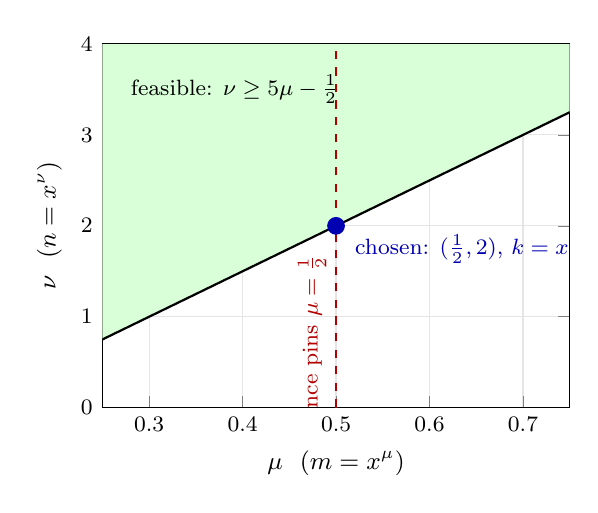
\begin{tikzpicture}
\begin{axis}[
  width=0.62\textwidth, height=6.2cm,
  xmin=0.25, xmax=0.75, ymin=0, ymax=4,
  xlabel={$\mu$ \ ($m=x^{\mu}$)}, ylabel={$\nu$ \ ($n=x^{\nu}$)},
  tick label style={font=\footnotesize}, label style={font=\small},
  grid=major, grid style={gray!20}]
\addplot[name path=lo, domain=0.25:0.75, thick, black] {5*x-0.5};
\addplot[name path=top, domain=0.25:0.75, draw=none] {4};
\addplot[green!15] fill between[of=lo and top];
\addplot[only marks, mark=*, mark size=3pt, blue!70!black] coordinates {(0.5,2)};
\node[font=\footnotesize, anchor=west, blue!70!black] at (axis cs:0.51,1.75) {chosen: $(\tfrac12,2)$, $k=x^{9/2}$};
\node[font=\footnotesize, anchor=west] at (axis cs:0.27,3.5) {feasible: $\nu\ge 5\mu-\tfrac12$};
\draw[dashed, red!70!black, thick] (axis cs:0.5,0) -- (axis cs:0.5,4);
\node[font=\footnotesize, red!70!black, rotate=90, anchor=south] at (axis cs:0.5,0.6) {balance pins $\mu=\tfrac12$};
\end{axis}
\end{tikzpicture}
\caption{Exponent bookkeeping. The word count ($\kappa\ge 5\mu+\nu$) and term T4 ($\kappa\le
2\nu+\tfrac12$) only require $\nu\ge 5\mu-\tfrac12$; any point of the shaded region is a valid family.
Only the balance of Figure~\ref{fig:balance} picks $\mu=\tfrac12$.}\label{fig:exponents}
\end{figure}



\begin{remark}[\Reading]
Since $\Gz(x)=\Omega(\sqrt{x})$, no valid argument can push $m$ beyond $\sqrt{x}$ and win. As far as
the constraints above go, the family could be built with $m=x^{1/2+\delta}$; so the barrier must be
paid on the error side, in T3. Section~\ref{sec:D} locates it.
\end{remark}

% ======================================================================
\section{Step D: the divisibility layer}\label{sec:D}
% ======================================================================

\subsection{The abstract data and the pointwise bound}

The size layer works with a record \lean{Data} of real numbers and a bundle of hypotheses
\lean{SizeData_2}: \lean{DIV}, \lean{EComp5}, \lean{HComp}, \lean{Count5}, \lean{Slopes},
\lean{QuotientSlopeBoundsWith}, \lean{LossBounds}, \lean{SlopeIneq}, \lean{HHBound}, \lean{FParams}.
No automorphic objects appear there. \lean{ChainTied} (\lean{TieGlobal.lean:97}) attaches the record
to an arithmetic family \lean{FamP} through \lean{TiePts}, \lean{TieGlobal}, \lean{TieLocal},
\lean{TieArith}; it is produced by \lean{linkCore} from fourteen family hypotheses, and only the
caller \lean{linkGLOBAL7_items} is used (\Exact).

\begin{theorem}[\lean{each_unit_bound_statement}, \Exact]
For every point $u_0$: $\ASK(u_0)\le\MAIN(u_0)+\mathrm{ErrX5at}(u_0)$.
\end{theorem}

\begin{figure}[ht]
\centering
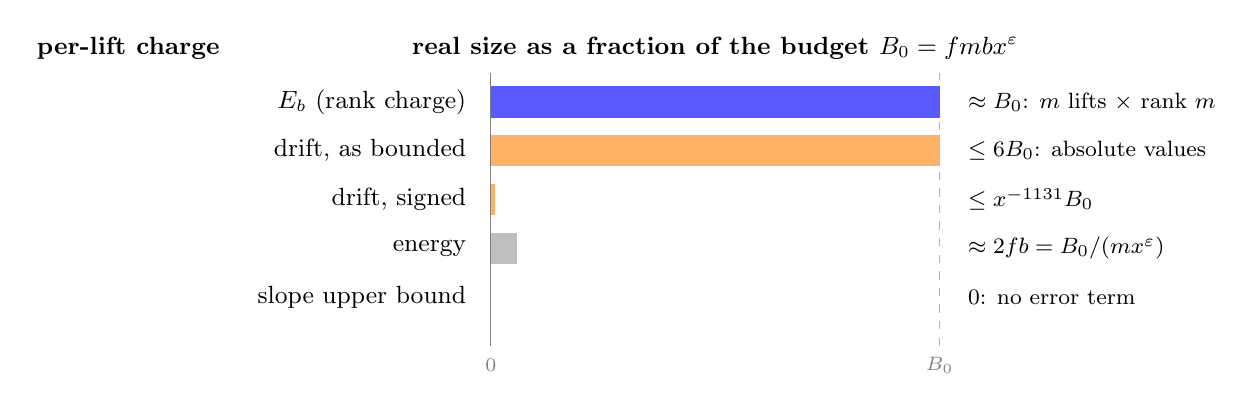
\begin{tikzpicture}[x=0.95cm, y=0.62cm]
\node[font=\small\bfseries, anchor=west] at (-6.2,6.1) {per-lift charge};
\node[font=\small\bfseries] at (3,6.1) {real size as a fraction of the budget $B_0=fmbx^{\eps}$};
\draw[gray] (0,0) -- (0,5.6); \draw[gray!60, dashed] (6,0) -- (6,5.6);
\node[font=\scriptsize, gray] at (6,-0.4) {$B_0$}; \node[font=\scriptsize, gray] at (0,-0.4) {$0$};
\foreach \y/\name/\len/\col/\note in {
  5/{$E_b$ (rank charge)}/6/blue!65/{$\approx B_0$: $m$ lifts $\times$ rank $m$},
  4/{drift, as bounded}/6/orange!60/{$\le 6B_0$: absolute values},
  3/{drift, signed}/0.05/orange!60/{$\le x^{-1131}B_0$},
  2/{energy}/0.35/gray!50/{$\approx 2fb = B_0/(mx^{\eps})$},
  1/{slope upper bound}/0/gray!50/{$0$: no error term}}{
  \node[font=\small, anchor=east] at (-0.2,\y) {\name};
  \ifdim \len pt>0pt \fill[\col] (0,\y-0.32) rectangle (\len,\y+0.32); \fi
  \node[font=\footnotesize, anchor=west] at (6.25,\y) {\note};
}
\end{tikzpicture}
\caption{What each per-lift charge really costs (Section~\ref{sec:D}). Only $E_b$
uses its budget; the drift's full size is an artefact of taking absolute values, and the energy and
slope budgets are almost empty. Bars are schematic: the energy bar would be invisible at true scale.}\label{fig:charges}
\end{figure}



The terms of $\mathrm{ErrX5at}$ that matter (\Verified, \lean{QuotientSlopeBoundsWith.lean:45}):

\begin{center}
\renewcommand{\arraystretch}{1.15}
\begin{tabular}{@{}llll@{}}
\toprule
Term & From & After dividing by $n_Tmb$ & Balance\\
\midrule
$c_{Div}\,n_T\,a\,L_a$ & \lean{DIV} & $\approx x/m$ & T1\\
$c_{Div}\,m(B_0+N_c)x^{e_{Div}\eps}$ & \lean{DIV} & $\approx m$ & T3\\
$m\,c_E\,B_0$ & \lean{EComp5} & same order & (slack)\\
$c_{Sl1}\,m\,B_0$ & \lean{QuotientSlopeBoundsWith} & same order & (slack)\\
$c_{Slope}\,n_T a L_a(1+m/k)$ & bookkeeping & $x/m(1+m/k)$ & T1, T2\\
\bottomrule
\end{tabular}
\end{center}

\subsection{The slope layer and the cancellation of the main terms}

\Verified{} \lean{EComp5} says $|E_e(u_0,u)-m\cdot\mathrm{sumA}\cdot\mathrm{lg}|\le c_E\, m\, B_0$:
the chain energy is $m$ copies of one step's slope, $\mathrm{lg}=\log(g_0g_1)$ for the two host
primes. \lean{Ga_bound5} combines the upper bound
$E_e\le m(\mathrm{sumA}\cdot\mathrm{lg}+c_EB_0)$ with \lean{key_identity5}, which contains
$+m\cdot\mathrm{sumA}\cdot\mathrm{lg}$; the main terms cancel exactly and the proof ends in
\texttt{linarith}. This is the ``cancellation of order-$m$ terms'' of the outline (entry~9).

\subsection{The local energy and why its budget is slack}

\Verified{} The energy is pinned by \lean{SizeData_2.EDef}: $E(u,j,w)=\mathrm{Eval}(u,j,w)$, a case
split on the residue characteristic of the place $w$:

\begin{center}
\renewcommand{\arraystretch}{1.15}
\begin{tabular}{@{}p{38mm}p{78mm}l@{}}
\toprule
$w$ lies over & $E(u,j,w)$ & depends on $j$?\\
\midrule
$T_u$ (auxiliary prime of $u$) & twice the weight deviation $+\ f\cdot N_m + \dots$ & no\\
$g_0$ or $g_1$ (host primes) & $v_p(D_\Gamma)+\mathrm{FTypeG}(j)+v_{NN}+c_g f(N_m^2+m^2\eta_{Sz})$ & yes\\
ramified class at $d$ & $v_p(D_\Gamma)+\mathrm{FRamD}(j)+\dots$ & yes\\
small $p\le X''$ & $v_p(D_\Gamma)+$ log terms & yes\\
other & $v_p(D_\Gamma)$ & no\\
\bottomrule
\end{tabular}
\end{center}

At $g_i$, with $\pi_{g_i}\bar\pi_{g_i}=g_i$ in the CM field,
$v_{NN}=\bigl(\sum_\tau \mathrm{nuAbs}(u,j,\tau)\,v_w(\tau(\bar\pi_{g_i}))\bigr)/e_w$.

\begin{proposition}[Per-lift energy, \Exact{} chain]
\lean{EComp} per lift (\lean{adm11}) follows from
\begin{itemize}
\item \lean{NormDecompositionCond}: $\sum_{w\mid g_i} sz(w,v_{NN}) = \bigl(\sum_\tau\mathrm{nuAbs}(u,j,\tau)\bigr)\log g_i$ (an exact equality);
\item \lean{factEtaMean}: $\sum_{w\mid \ell}\mathrm{lw}(w)e_w = \log \ell$ (product formula);
\item \lean{DegreeCountBound}: $\bigl|\sum_\tau\mathrm{nuAbs} - \mathrm{fockDeg}(j) - \sum_t a_T(t)\bigr|\le \mathrm{errG}(j)$;
\item \lean{TypePrimeSizeBound} and the off-$g$ bounds.
\end{itemize}
\end{proposition}

\paragraph{The row structure.} \Verified{} (\lean{nuAbs_place_fine}) At lift $j=i+1$ and an
archimedean place $\tau$, nuAbs sums $N(j-1)=k+i(t+1)$ rows
$\mathrm{nuRow}(u,j,\tau,r)=\mathrm{srcPar}(u,\tau,r)+w_{Sz}(j,\tau)-\tfrac12(N(j-1)+N(j)-1-2r)$:
the two end rows carry top and off-top weights, the middle rows are $\approx w_j(j,\tau)$, and the
$i(t+1)$ block rows are $\approx 0$ up to $2\eta_{Sz}$.
\Reading{} A parameter plus a weight minus a $\rho$-type half-sum looks like the Harish-Chandra
parameters at lift $j$; \lean{kerPlace} sums $\phi(\nu)=\nu\log\nu-\nu$ over the rows, a Stirling
shape.

\paragraph{The $g$-place energy bound.} \Verified{} (\lean{linkDIVt_of_rowsF},
\lean{secondComplement_of_split}, \lean{WeightDegreeSizes.lean:142--261}) The $g$-place energy
clause of \lean{LinkDIV_at} is not a global product formula across all places, but a local sum
over the places $w\mid g_i$ ($i\in\{0,1\}$, combined via $\log(g_0g_1)=\log g_0+\log g_1$ in
\lean{prod_gTypes}). Specifically, \lean{NormDecompositionCond} gives
$\sum_{w\mid g_i}\mathrm{sz}(w,v_{NN})=(\sum_\tau\mathrm{nuAbs}(u,j,\tau))\log g_i$,
\lean{factEtaMean} cancels the Fock-degree offset $2\,\mathrm{FTypeG}=-\mathrm{fockDeg}$,
\lean{DegreeCountBound} bounds $|\sum_\tau\mathrm{nuAbs}-\mathrm{fockDeg}-\sum_t a_T|\le\mathrm{errG}(j)$,
and \lean{TypePrimeSizeBound} absorbs $(\mathrm{errG}(j)+2v_{g_i}(D_\Gamma)+2\,\mathrm{er})\log g_i\le C B_0$.

\begin{proposition}[\Ours]
The real per-lift energy error is $\mathrm{errG}(j)\approx 2\sum_\tau w_j(j,\tau)\approx 2fb$,
with no factor $m$, against a budget $B_0=f\,m\,b\,x^\eps$. The energy charge $m\,c_E B_0$ therefore
has a spare factor of about $m x^\eps$. The slope upper bound is \lean{ClaimHigh}:
$\mu_{\max}(N)\le\mu_{\max}(M)+G_a+F_o-E_e$ with \emph{no} error term; \lean{slopesN_at_of} adds the
$m B_0$ allowance from $0\le C m B_0$ alone.
\end{proposition}

\subsection{The divisibility inequality}

\begin{theorem}[\lean{Data.DIV}, \Exact]\label{thm:DIV}
\begin{multline*}
\mu_{CC}+h(u)-F_o \le \sum_t\Bigl(m\bigl(\phi(a_T(t))-a_T(t)\log\Omega\bigr)-a_T(t)\log T(u)\Bigr)\\
+ c_{Div}\,n_T\,a\,L_a + c_{Div}\,m\,(B_0+N_c)\,x^{e_{Div}\eps}.
\end{multline*}
\end{theorem}

\paragraph{The height of a chain.} \Verified{} (\lean{height_chain_atR}) The pairing map $B_u$
factors through a chain of $m$ maps $K_j$, one per lift, with $\|K_j\|_v^2\le\exp(h_K(j,v))$, and
\[
\log\|B_u\|_v^2\le h_P+\sum_{j=1}^m h_K(j,v)-\log\kappa_v-\min_p\sum_j\log\lambda_j(p,v).
\]
This is submultiplicativity of operator norms along the chain. \Reading{} It is where ``a chain of
theta lifts'' becomes an inequality.

\paragraph{The per-lift charge is built in.} \Verified{} (\lean{ZscOfNum}, \lean{errB_of_units})
The scale data sets, per lift, an error unit $E_{1u}=x^\eps(B_0+N_c)$, a main term
$l_{3m}(j)=\sum_\rho[(k+j-1)-(m-j)]\,w(j,\rho)\log\Omega$ (the signature difference $p_j-q_j$ times
the weights) and $l_{3u}=B_0\log\log x$. Summing over $m$ lifts gives the $m\,x^\eps(B_0+N_c)$ term.

\paragraph{Absorption.} \Verified{} (\lean{divisor_inequality_assembly}, \lean{error_absorption})
Every error term inside \lean{DIV} is bounded against $m(B_0+N_c)x^\eps$:

\begin{center}
\renewcommand{\arraystretch}{1.15}
\begin{tabular}{@{}lll@{}}
\toprule
Error term & Bound used & Versus the budget $mB_0x^\eps$\\
\midrule
$\sum e_E$ (place heights) & $15C_0 f m b L$ & spare factor $\approx m$\\
$\sum|\delta||\log\Omega|$ & $15C_0fmbL + C_0n_TaL_a$ & spare factor $\approx m$\\
$\sum e_K$ (per-lift polynomial) & $5C_0 m f b L$ & spare factor $\approx m$\\
$e_6,e_P,L_{pass}$ & $\le B_0$ & spare factor $\ge m$\\
$\sum|pq_j-k||w||\log\Omega|$ (drift) & $6mB_0$ & full budget\\
$E_b$ (rank charges) & hypothesis $C_0mx^\eps(B_0+N_c)$ & full budget\\
\bottomrule
\end{tabular}
\end{center}

\subsection{The signature drift is an artefact}

\begin{proposition}[\Ours]\label{prop:drift}
The drift term is smaller than the bound used for it by a factor of at least $x^{1131}$.
\end{proposition}

\begin{proof}
\Verified: $pq_j=(k+j-1)-(m-j)$, so $pq_j-k=2j-1-m$ (\lean{NumbersLink.lean:574}). The proof bounds
each term $(pq_j-k)\,w(j,\rho)\log\Omega$ by its absolute value \emph{before} summing (step
\texttt{hA} of \lean{divisor_inequality_assembly}). By \lean{SizeData_2.be_close},
$|w(j,\rho)-w(j',\rho)|\le 2\eta$ for all lifts, and \lean{szRow_eta_bounds} gives
$\eta\le b/(t^3fk^3)$. Since $\sum_{j=1}^m(2j-1-m)=0$,
\[
\sum_j\sum_\rho(2j-1-m)\,w(j,\rho)\log\Omega=\log\Omega\sum_\rho\sum_j(2j-1-m)\bigl(w(j,\rho)-w(1,\rho)\bigr),
\]
so the signed drift is at most $L_a f(m^2/2)2\eta=fm^2\eta L_a$, while the absolute bound used is
$2fm^2bL_a$. The ratio is at most $\eta/(2b)\le 1/(2t^3fk^3)\le x^{-1131}$ since $t\ge x^{377}$.
\end{proof}

\begin{figure}[ht]
\centering
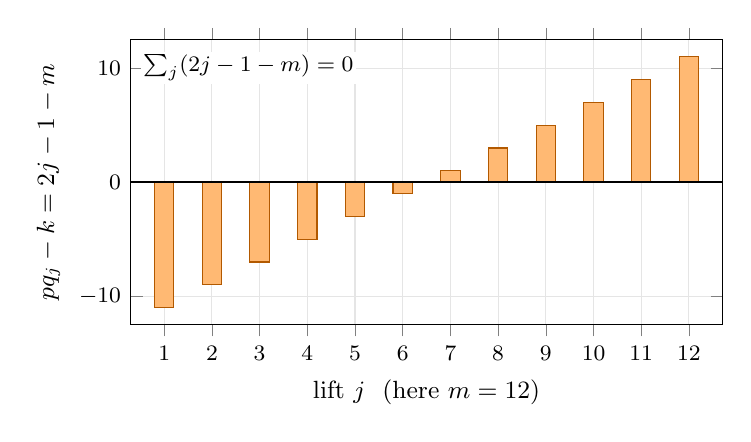
\begin{tikzpicture}
\begin{axis}[
  width=0.75\textwidth, height=5.2cm, ybar, bar width=7pt,
  xmin=0.3, xmax=12.7, ymin=-12.5, ymax=12.5,
  xlabel={lift $j$ \ (here $m=12$)}, ylabel={$pq_j-k=2j-1-m$},
  xtick={1,...,12}, tick label style={font=\footnotesize}, label style={font=\small},
  grid=major, grid style={gray!20}]
\addplot[fill=orange!55, draw=orange!70!black] coordinates {(1,-11) (2,-9) (3,-7) (4,-5) (5,-3) (6,-1) (7,1) (8,3) (9,5) (10,7) (11,9) (12,11)};
\draw[thick] (axis cs:0.3,0) -- (axis cs:12.7,0);
\node[font=\footnotesize, anchor=north west, fill=white, inner sep=1pt] at (axis cs:0.5,11.5) {$\sum_j(2j-1-m)=0$};
\end{axis}
\end{tikzpicture}
\caption{The signature drift. Its coefficients sum to zero and the weights $w(j,\rho)$ agree across
lifts up to $2\eta$, so the signed drift nearly cancels. The proof bounds each bar by its absolute
value instead, which is where its nominal $m^2$ comes from.}\label{fig:drift}
\end{figure}



\subsection{The rank bound $E_b$: where the $m^2$ really lives}

\begin{theorem}[\Ours, each step \Verified]\label{thm:Eb}
$E_b\approx m\cdot B_0$, and both factors of $m$ are structural.
\end{theorem}

\begin{sketch}
\begin{enumerate}
\item \emph{The outer $m$ is the number of lifts.} \lean{errB_of_units} sums over $J$ with
  $|J|=m$ (\lean{RecNums.p12}).
\item \emph{The real obligation.} $E_{1u}$ is set by definition; the content is the field
  \lean{IndefData.ON}: for each lift $j$,
  $\sum_{w\in T_w}\log w\,(\mathrm{ram}_w\,\mathrm{err}_0(w,j)+\mathrm{ram}_w J_0(w,j))\le E_1(j)$,
  supplied on the family side by \lean{DIVinN_at} and \lean{LinkN_at}:
  $\mathrm{etaSum}(j)\le d_{Z0}(j)\bigl(C(fmbL^2+\log^2x\,N_c)+\sum_\ell\mathrm{vvTerm}(\ell)\bigr)$.
  The last sum is the $\Sha$ loss of Section~\ref{sec:F}, added once and bounded by $\sqrt b$.
\item \emph{No double counting.} \lean{linkN_of_gd} bounds $\mathrm{etaSum}(j)$ through
  $\mathrm{etaJ}(j,w)=\sum_{i\in\mathrm{locs}(j,w)}\mathrm{etaLoc}(i)$, and by
  \lean{NData.locs_mem}, $i\in\mathrm{locs}(j,w)\iff j(i)=j\wedge w(i)=w$: every local piece
  belongs to exactly one lift.
\item \emph{The inner $m$ is a Bloch--Kato rank.} The allowance at a small prime $\ell$ is
  $\mathrm{costC}(\ell)=6000\,f\,m\,h_B\,\mathrm{sl}(\ell)+30000f^2t^2n_V\,(\dots)$ with
  $h_B=b+S_c+\eta_{Sz}+t+2\in[b,6b]$. The colength bound behind it calls \lean{rank_le_row} with
  $m:=D.R.m$:
  \[
  \dim H^1_f(K_w,T)\le\mathrm{locDeg}(w)\cdot m,
  \]
  the Bloch--Kato count~\cite{bloch-kato} $\dim H^1_f=\sum_\tau\#\{\text{non-negative Hodge--Tate weights}\}$, and the
  family supplies the hypothesis $|L_o|\le m$ by \emph{equality} (\lean{le_of_eq}), from its weight
  pattern \lean{ShapeJumps k m t}.
\end{enumerate}
\end{sketch}

\begin{center}
\renewcommand{\arraystretch}{1.15}
\begin{tabular}{@{}lll@{}}
\toprule
Factor of $E_b$ & Source & Size\\
\midrule
number of lifts & $|J|=m$ & $m$\\
rank per piece & Bloch--Kato, fixed by equality & $m\cdot\mathrm{locDeg}$\\
exponent per piece & lift exponent $e'$ & $\approx b$\\
primes & $\sum\log\ell$ over small primes & $\approx x^\eps$\\
$\Sha$ loss & $\sum\mathrm{vvTerm}\le\sqrt b$, once per lift & negligible\\
\bottomrule
\end{tabular}
\end{center}

\paragraph{Why the two $m$'s are one $m$. \Ours}
\Verified{} \lean{ShapeJumps k m t} (\lean{EmbeddingTypes.lean:99}), required by \lean{admG2} at every
small prime, place and embedding, says the Hodge--Tate multiplicity of the twisted lifted
representation is the indicator of $C\cup L\cup[0,t)$: $k-1$ weights in a far cloud $C$, exactly $m$
weights $L$ near $0$, and the $t$-block $[0,t)$ from cyclotomic twists $\chi^c$, $c=1,\dots,t$. With
$r=k+m-1$ and $n_V=r+t$, the weights $C\cup L$ have sizes $(k-1,m)$: the starting signature.
\Reading{} The $m$ low weights are the indefinite side of the signature, and the chain has exactly
$m$ lifts because it walks that side down to $0$. So $E_b$'s $m^2$ is one $m$ used twice, by
construction.

\begin{figure}[ht]
\centering
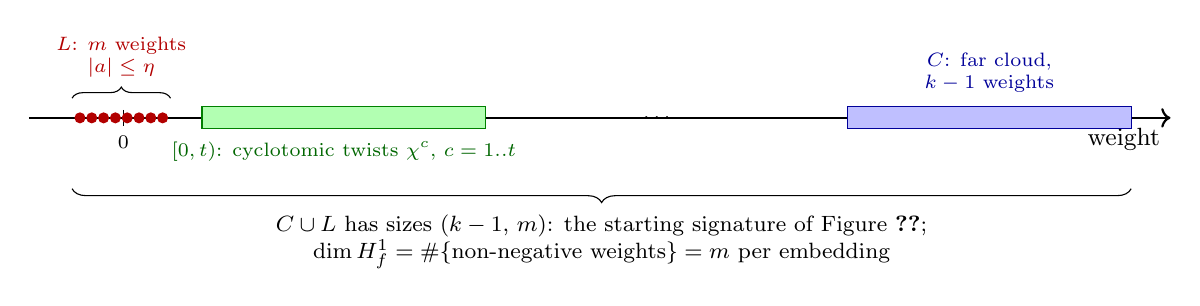
\begin{tikzpicture}[x=1cm]
\draw[->, thick] (-1.2,0) -- (13.3,0) node[below left, font=\small] {weight};
\draw (0,0.1) -- (0,-0.1) node[below, font=\scriptsize] {$0$};
\foreach \x in {-0.55,-0.4,-0.25,-0.1,0.05,0.2,0.35,0.5} \fill[red!70!black] (\x,0) circle (2pt);
\draw[decorate, decoration={brace, amplitude=4pt}] (-0.65,0.25) -- (0.6,0.25) node[midway, above=4pt, font=\scriptsize, align=center, red!70!black] {$L$: $m$ weights\\ $|a|\le\eta$};
\fill[green!30] (1.0,-0.14) rectangle (4.6,0.14); \draw[green!50!black] (1.0,-0.14) rectangle (4.6,0.14);
\node[font=\scriptsize, below, green!40!black] at (2.8,-0.18) {$[0,t)$: cyclotomic twists $\chi^c$, $c=1..t$};
\node[font=\scriptsize] at (6.8,0.0) {$\cdots$};
\fill[blue!25] (9.2,-0.14) rectangle (12.8,0.14); \draw[blue!60!black] (9.2,-0.14) rectangle (12.8,0.14);
\node[font=\scriptsize, above, blue!60!black, align=center] at (11,0.2) {$C$: far cloud,\\ $k-1$ weights};
\draw[decorate, decoration={brace, amplitude=5pt, mirror}] (-0.65,-0.9) -- (12.8,-0.9)
  node[midway, below=6pt, font=\footnotesize, align=center] {$C\cup L$ has sizes $(k-1,\,m)$: the starting signature of Figure~\ref{fig:chain};\\
  $\dim H^1_f=\#\{\text{non-negative weights}\}=m$ per embedding};
\end{tikzpicture}
\caption{The weight pattern \texttt{ShapeJumps k m t} (schematic, not to scale). The $m$ low weights
are both the indefinite part of the starting signature and the Bloch--Kato rank of each piece.}\label{fig:weights}
\end{figure}



\paragraph{Where $b$ enters. \Verified}
The lift exponent is
$e'=e_L(\ell,N,h)=32(2h\,s_N(\ell,N)+1)+\lambda_N(\ell,N,h)$ with $h=\lfloor h_B\rfloor$, linear in
a height $h_B\in[b,6b]$. \Reading{} A lifting exponent growing linearly with the Hodge--Tate height,
as in Fontaine--Laffaille-type bounds. Since both the main term $n_Tmb$ and the cost $mB_0$ are linear
in $b$, \textbf{$b$ cancels in the balance}: $e'\approx b$ sets the absolute size of $E_b$, not its
dependence on $m$.

\subsection{The $+m$ side of the balance is the divisibility error}

\begin{theorem}[\Ours, pieces \Verified]
Both sides of the balance $x/m+m$ come from \lean{DIV}: the $x/m$ term from $c_{Div}n_TaL_a$ (top
weights $a=xb$), the $m$ term from $c_{Div}m(B_0+N_c)x^{e_{Div}\eps}$, which on the lattice side is
$\mathrm{errB}=\text{drift}+E_b$.
\end{theorem}

\begin{remark}[\Verified, unused route]
\lean{exists_data_completion} (\lean{PChain.lean:306}), proved but not used, builds from the single
bound $\ASK\le\MAIN+c_{Div}n_TaL_a+c_{Div}m(B_0+N_c)x^{e_{Div}\eps}+L_{oP}$ a degenerate data record
(one word per point, zero energy) satisfying all of \lean{SizeData_2}. So even with zero energy and
slope charges, the divisibility error alone gives T3.
\end{remark}

\begin{corollary}[\Reading]
With the drift an artefact (Proposition~\ref{prop:drift}) and the energy and slope budgets slack, the
reason the chain is cut at $m\approx\sqrt{x}$ rests on one term: $E_b$, $m$ lifts times a Bloch--Kato
rank of $m$ per piece. This is consistent with $\Gz(x)=\Omega(\sqrt{x})$.
\end{corollary}

\subsection{The common lattice}\label{sec:RR}

\begin{proposition}[\lean{exists_divStage_of_pk}, \Exact; \Ours{} as the answer to Whidden's question]
The single lattice $RR$ shared by all words is
\[
x\in RR.L\iff \forall w\ \exists d\in\Oc_{LL},\ d\notin\mathfrak p_w,\ \ d\,x\in\Oc_{LL}\text{-span}\{y : j_E y\in \mathrm{RRset}(\mu_w)\},
\]
where $\mathrm{RRset}(\mu)=\iota_\mu(\Lambda_\mu)$, $\iota_\mu=\mathrm{multZero}\circ\mathrm{downTo}_{\mu,m}\circ\mathrm{multTop}^{-1}$
is the composite of the $m$ lift steps, and $\mu_w=\texttt{muAt }w$ is the $\xi$-twist data at $w$
(\lean{prescribedRowLat}).
\end{proposition}

So $RR$ is the intersection over places of the localisations built from each place's own character
twist: a lattice gcd. Every family carries it as the field \lean{FamP.rrDef : DV.RRDef}.

\begin{figure}[ht]
\centering
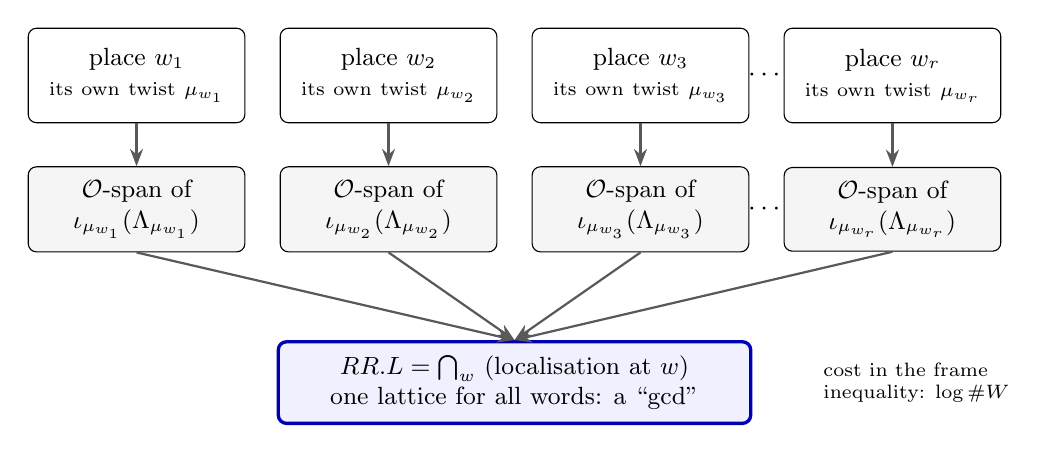
\begin{tikzpicture}
\foreach \i/\x/\nm in {1/0/w_1,2/3.2/w_2,3/6.4/w_3,4/9.6/w_r}{
  \node[fbox, text width=24mm, minimum height=12mm] (p\i) at (\x,0)
    {place $\nm$\\ {\scriptsize its own twist $\mu_{\nm}$}};
  \node[fbox, fill=gray!8, text width=24mm] (l\i) at (\x,-1.7) {$\Oc$-span of\\ $\iota_{\mu_{\nm}}(\Lambda_{\mu_{\nm}})$};
  \draw[farr] (p\i) -- (l\i);
}
\node at (8.0,0) {$\cdots$}; \node at (8.0,-1.7) {$\cdots$};
\node[fbox, hl, minimum width=60mm] (RR) at (4.8,-3.9) {$RR.L=\bigcap_w$ (localisation at $w$)\\ one lattice for all words: a ``gcd''};
\foreach \i in {1,2,3,4} \draw[farr] (l\i.south) -- (RR.north);
\node[font=\scriptsize, align=left, anchor=west] at (8.6,-3.9) {cost in the frame\\ inequality: $\log\#W$};
\end{tikzpicture}
\caption{The common lattice $RR$ (\texttt{prescribedRowLat}). Each place contributes the image of its
own integral points under the composite of the $m$ lift steps, built from its own character twist;
$RR$ is their intersection.}\label{fig:RR}
\end{figure}


\Reading{} This matches the outline's entry~15 (``glue an integral structure across Hecke characters
for a gcd''). Its only visible cost is $\log\#W$ in the frame inequality.

\subsection{The degree identity: how a slope becomes $\ASK-\MAIN$}

There is no single lemma; it is a chain of four used statements.

\begin{figure}[ht]
\centering
\begin{tikzpicture}[node distance=7mm]
\node[fbox, text width=46mm, fill=orange!8] (fin) {\textbf{finite places}\\ gain $\ge$ prime counts\\ $\ASK-L_{oP}\le G_a$ \ (\textbf{2})};
\node[fbox, text width=46mm, right=14mm of fin] (slope) {\textbf{Arakelov slope}\\ $\mu(Nu)\approx\mu(NuH)+G_a+F_o-E_e$ \ (\textbf{1})};
\node[fbox, text width=46mm, below=10mm of slope] (frame) {\textbf{slope inequality on $RR$}\\ $\mathrm{mean}_u[\mu(Nu)-h_u]\le\mu_{dual}(RR)+\log\#W$ \ (\textbf{4})};
\node[fbox, text width=46mm, left=14mm of frame, fill=green!8] (inf) {\textbf{infinite places}\\ periods (Chowla--Selberg)\\ $\mu_{dual}+h-F_o\le\MAIN+\Err$ \ (\textbf{3})};
\node[fbox, hl, text width=60mm, below=10mm of $(inf.south)!0.5!(frame.south)$] (res) {$\ASK\le\MAIN+\Err$\\ {\scriptsize (after the $m\cdot\mathrm{sumA}\cdot\mathrm{lg}$ terms cancel in \lean{Ga_bound5})}};
\draw[farr] (fin) -- (slope);
\draw[farr] (slope) -- (frame);
\draw[farr] (frame) -- (inf);
\draw[farr] (inf.south) -- (res);
\end{tikzpicture}
\caption{The degree identity. The Arakelov degree of the divisible lattice is computed at the finite
places (where the prime counts $\ASK$ enter) and at the infinite places (where the periods $\MAIN$
enter); the slope inequality on the one common lattice joins them.}\label{fig:degree}
\end{figure}



\begin{enumerate}
\item \textbf{Slope $=$ reference $+$ local indices} (\lean{NprimeMuR}, supplied through
  \lean{LinkMu} $\Leftarrow$ \lean{J.linkMu_of_linkDIV} $\Leftarrow$ \lean{LinkDIV}):
  \begin{gather*}
  \Bigl|\mu(Nu\,u)-\mu(NuH\,u)-\sum_{w\in\mathrm{supp}} sz(w,sg(u,w))\Bigr|\le C X'',\\
  sg(u,w)=\sum_j\bigl(\mathrm{gain}_j(w)+F_j(w)-E(u,j,w)\bigr),
  \end{gather*}
  with $sz(w,y)=2\,\mathrm{lw}(w)\,e_w\,y$. Summed: $\mu(Nu\,u)\approx\mu(NuH\,u)+G_a+F_o-E_e(u)$.
\item \textbf{Gain $\ge$ prime count} (\lean{LinkG_at}, where $\ASK$ enters). At an inert place $w$
  over $p\le X''$:
  \[
  \sum_j\sum_t\bigl(\mathrm{vMCS}_{j,t}(p)-\mathrm{loss}\bigr)-m\,\mathrm{fl}(p)\le\sum_j\mathrm{gain}_j(w)-\tau(w),
  \]
  \[
  \mathrm{vMCS}_{j,t}(p)=\sum_{i\text{ odd}}\max\bigl(0,\,a_t/p^i-\mathrm{wPart}(j,t,p,i)\bigr).
  \]
  This is a Legendre-type count, like $v_p(a!)=\sum_i\lfloor a/p^i\rfloor$ but over odd $i$ with
  weights removed. Since
  $\ASK=\sum_j\sum_t\bigl(\sum_{p\text{ inert}}2\log p\cdot\mathrm{vMCS}_{j,t}(p)+\dots\bigr)$, summing
  over $w\mid p$ with the product formula gives $\ASK-G_a\le L_{oP}$ (\lean{loss_bound_at}).
\item \textbf{Dual slope $\le$ period term} (\lean{LinkDIV_at}, where $\MAIN$ enters):
  \[
  \mu_{dual}(RR)+h(u)-F_o\le\MAIN(u)+C|T_T|aL_a+Cm(B_0+N_c)x^{C_{abs}\eps},
  \]
  \[
  \MAIN(u)=\sum_t\bigl[m(\phi(a_t)-a_t\log\Omega)-a_t\log T_u\bigr],\qquad
  \log\Omega=\gamma+\log(\pi/v)-\frac{L'}{L}(1,\chi_d),
  \]
  the Chowla--Selberg period~\cite{chowla-selberg} (\lean{meanPeriod}), and $\phi(a)=a\log a-a$.
\item \textbf{Slope inequality} (\lean{Frame_at}): the rank-weighted mean $s$ of
  $\mu(Nu\,u)-h_u$ satisfies $s-\log\#W-(\text{small})\le\mu_{dual}(RR)$, for the one lattice $RR$
  of Section~\ref{sec:RR}.
\end{enumerate}

\begin{theorem}[Assembled, \Reading{} with each step \Verified]
\[
\ASK-L_{oP}\le G_a,\qquad
\mu(Nu\,u)\approx\mu(NuH\,u)+G_a+F_o-E_e(u),
\]
\[
\operatorname{mean}_u[\mu(Nu\,u)-h_u]\le\mu_{dual}(RR)+\log\#W,
\]
\[
\mu_{dual}(RR)+h(u)-F_o\le\MAIN(u)+\text{errors}
\quad\Longrightarrow\quad \ASK-\MAIN\le\text{errors},
\]
after the $m\cdot\mathrm{sumA}\cdot\mathrm{lg}$ main terms cancel in \lean{Ga_bound5}. The finite
part of the Arakelov degree of the divisible lattice is a sum of local indices bounded below by the
prime counts; the archimedean part is bounded by the CM period main term.
\end{theorem}

\subsection{Local divisibility: the $\sqrt p$ trick}

\begin{lemma}[\lean{key_minor_dvd}, \Exact]
Let $A$ be a commutative ring, $p$ prime, $w\in A$ with $w^2=p$. Let $M,N'$ be
$(k+1)\times(k+1)$ matrices over $A$ with $M_{ba}^{p^e}\equiv N'_{ba}\pmod p$ for all $b,a$, and let
$u,u'\in A^{k+1}$ with $w\mid u_b$ and $w\mid u'_b$ for $b\neq0$. Then for every column $c$,
\[
w\ \Big|\ \Bigl(\sum_b u'_bN'_{bc}\Bigr)\Bigl(\sum_b u_bM_{b0}\Bigr)^{p^e}-\Bigl(\sum_b u'_bN'_{b0}\Bigr)\Bigl(\sum_bu_bM_{bc}\Bigr)^{p^e}.
\]
\end{lemma}

\Exact{} Used chain: \lean{key_minor_dvd} $\to$ \lean{kW_ord} $\to$ \lean{key3Ord}
(\lean{CoarseMultiplicityOrderBound}: for $g\in GL$ over the Witt vectors $W(\mathbb F_{p^{n'}})$,
the key polynomials after the lift substitution lie in $W_1$) $\to$ \lean{third_key_of_order}
$\to$ \lean{restRawTail1_of} $\to$ \lean{stmtEExt_of_15c} (\lean{ExtendedClosedForm}) $\to$
\lean{extendedClosedForm}. \lean{LinkG} is assembled by \lean{link_of_local_closed} from the first
and second closed-form theorems and the local model results, all instantiated from one structure
\lean{Loc}, proved by \lean{loc_proved} from \lean{TraceSpectra.stmtE}.

\paragraph{The gain, orbit by orbit.} \Exact{} The gain clause of \lean{LinkG_at} is
\lean{AuxBlock8.Conclusion1}. It is proved from \lean{St.starAll_of}, one inequality per prime $p$,
lift $j$ and orbit representative $t_0$,
\[
\sum_{s\in\mathrm{tops}(t_0)}(\mathrm{askP}-\mathrm{lo})\le g_U+d_l-P_r-\lceil t_v\rceil-D_p-1,
\qquad
g_U=\gamma_p\sum_s\alpha(s)-\sum_s\sum_{e\text{ odd}}\min\bigl(\alpha(s)/p^e,\mathrm{cap}\bigr)-d_l,
\]
then summed (\lean{gain_bound_all_of_star}, \lean{gainBoundAll_add_one_of_gainBoundAllRequired}).

\begin{remark}[\Reading]
A congruence mod $p$ gives whole units of $p$. Working where $p$ has a square root extracts half a
unit per place, and the only valuation corrections in the gain are sums over \emph{odd} exponents,
the ones where a half unit shows. We did not trace the direct call from \lean{key3Ord} into $g_U$.
\end{remark}

% ======================================================================
\section{Step E: near-orthogonality of the words}\label{sec:E}
% ======================================================================

\begin{theorem}[\lean{LinkS_at}, \lean{LinkS}, \Exact]
If every word $u$ is comparable, $C_0^{-1}\le d_u(u)\Gamma^2/D^*\le C_0$, then
\begin{enumerate}
\item $\|K(u,u')\|_{HS}^2\le(1+\eta_0)\,d_u(u)d_u(u')/D^*$ for $u\neq u'$;
\item $\|K(u,u)-\mathrm{id}\|_{HS}^2\le e_0\,d_u(u)$;
\item $D_{all}\le(1+\eta_1)D^*$;
\end{enumerate}
with $\eta_0,\eta_1,\sqrt{e_0}\le\exp(-x^{\eps/8})$ and $\Gamma=\exp(C_\Gamma m^5fL)$.
\end{theorem}

\Verified{} The comparability premise is discharged where \lean{LinkS} is consumed:
\lean{matKF_of} feeds it \lean{ChosenProviso}, proved by \lean{chosenProviso_min} from the class
number formula (\lean{ClassNumberFormula_2}) and \lean{RankTiesF}. The bound itself comes from
\lean{theoremS_link_concrete}, from \lean{ResidEv}, \lean{RowsTieP}, \lean{CountAllPointsClass} and
four hypotheses \lean{ClKppOff} (the correction $K_{pp}$ vanishes off the diagonal),
\lean{ClKppDiag}, \lean{ClOff}, \lean{ClDiag}.

\Reading{} The normalised Gram matrix of the words is the identity up to $\exp(-x^{\eps/8})$. The
$m^5$ in $\Gamma$ is the same $m^5$ as the word count of Section~\ref{sec:windows}. This is the
``approximate orthogonality of columns'' of the outline (entry~16), and it does not touch the
balance.

% ======================================================================
\section{Step F: the $\Sha$ window and the classical inputs}\label{sec:F}
% ======================================================================

\begin{definition}[\lean{IsChiField}, \lean{VVle}]
For $e,q,d$ and a character $\psi$, a field $E\subset\Q(\zeta_N)$ is a $\chi$-field if it is fixed
exactly by the $a$ with $a\equiv\pm1\pmod{2^{e+2}}$, $\psi(a)=1$, $(a/q)=(a/d)=1$.
$\mathrm{VVle}(E,t,B)$ means: for every prime $\ell$ and $0<e<t$ the Tate--Shafarevich group
$\Sha_\ell(e)$ has finite length, and
\[
\sum_{\ell\in S}\log\ell\sum_{1\le e<t}\len\Sha_\ell(e)\le B\qquad\text{for every finite set } S.
\]
\end{definition}

\begin{theorem}[\lean{VWinAt psi 401}, \Exact]
For every $\eps\in(0,1/52)$ and page choice $e(x)$ with $x^{2+8\eps}\le 2^{e}\le 2x^{2+8\eps}$, there
are $J\ge1$ and $X_0$ such that for $X\ge X_0$ and every window pair $(q,d)$ there is $Y$ with
$X^{1/J}\le Y$, $Y^2\le X$, and for every $x\in[Y,Y^2]$ every $\chi$-field $E$ satisfies
$\mathrm{VVle}\bigl(E,\lfloor x^{401}\rfloor,\sqrt{\exp(x^\eps)}\bigr)$.
\end{theorem}

\Reading{} $E$ is the real $2^{e+2}$-cyclotomic layer cut by $\psi$ and the two auxiliary quadratic
characters, of degree about $2^e\approx x^{2+8\eps}\approx n$, matching the host. \lean{supplyChi}
turns the window into host existence for each character.

\paragraph{The proof chain.} \Exact{} One chain, all used:
\lean{vwin_of_row} $\to$ \lean{automorphic_window_of_inputs} $\to$
\lean{v_window_of_depth_zero_residual_bc_cm} $\to$ \lean{v_window_of_literal_automorphy_n} $\to$
\lean{v_window_of_automorphy_csd_ss_mono_odd} $\to$ \lean{vwin_of_hypotheses_H_E_alt} $\to$
\lean{of_four_alt} $\to$ \lean{vwin_of_counts} $\to$ \lean{vwin_of_joint} $\to$
\lean{vwinAt_of_joint}.

\begin{figure}[ht]
\centering
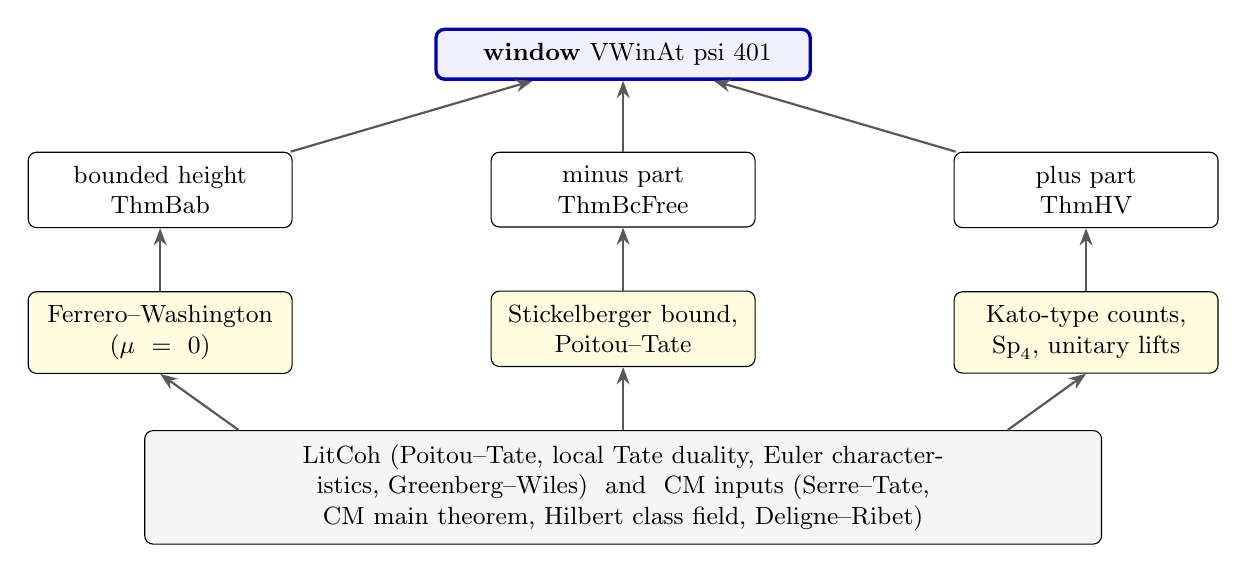
\begin{tikzpicture}[node distance=5mm]
\node[fbox, hl, text width=44mm] (V) {\textbf{$\Sha$ window} \lean{VWinAt psi 401}};
\node[fbox, text width=30mm, below left=9mm and 18mm of V] (B) {bounded height\\ \lean{ThmBab}};
\node[fbox, text width=30mm, below=9mm of V] (M) {minus part\\ \lean{ThmBcFree}};
\node[fbox, text width=30mm, below right=9mm and 18mm of V] (P) {plus part\\ \lean{ThmHV}};
\node[fbox, fill=yellow!12, text width=30mm, below=8mm of B] (FW) {Ferrero--Washington\\ ($\mu=0$)};
\node[fbox, fill=yellow!12, text width=30mm, below=8mm of M] (PT) {Stickelberger bound,\\ Poitou--Tate};
\node[fbox, fill=yellow!12, text width=30mm, below=8mm of P] (K) {Kato-type counts,\\ $\mathrm{Sp}_4$, unitary lifts};
\node[fbox, fill=gray!8, text width=118mm, below=8mm of PT] (L) {\lean{LitCoh} (Poitou--Tate, local Tate duality, Euler characteristics, Greenberg--Wiles) \ and \ CM inputs (Serre--Tate, CM main theorem, Hilbert class field, Deligne--Ribet)};
\foreach \a in {B,M,P} \draw[farr] (\a) -- (V);
\draw[farr] (FW) -- (B); \draw[farr] (PT) -- (M); \draw[farr] (K) -- (P);
\draw[farr] (L.north) -- (PT.south);
\draw[farr] (L.north west) ++(1.2,0) -- (FW.south);
\draw[farr] (L.north east) ++(-1.2,0) -- (K.south);
\end{tikzpicture}
\caption{What the $\Sha$ window rests on. All yellow and grey inputs are proved in Lean from one
\texttt{OpenImageCondition}; none is assumed.}\label{fig:sha}
\end{figure}



\begin{center}
\renewcommand{\arraystretch}{1.15}
\begin{tabular}{@{}p{50mm}p{95mm}@{}}
\toprule
Input & Rests on\\
\midrule
bounded-height part (\lean{ThmBab}) & \lean{thmBab_of_lemmaK} with \lean{ferreroWashington}\\
minus part (\lean{ThmBcFree}) & a Stickelberger-type bound
  $\len\Sha^-\log\ell\le C\ell[E:\Q]^2(e+1)\log(e\ell N)^2$, via \lean{ML.iv} (Poitou--Tate and unramified orthogonality)\\
plus part (\lean{ThmHV}) & counts I, II, III, V, Z and \lean{LemmaK}: Kato-type bounds, $\mathrm{Sp}_4$ inputs, unitary lifts\\
duality (\lean{LitCoh}) & Poitou--Tate, local Tate duality, local and global Euler characteristics, local and global finiteness, Greenberg--Wiles\\
CM inputs (\lean{LiteratureCMHypothesis}) & Grothendieck deformation, de Rham comparison, Serre--Tate, CM main theorem, Hilbert class field via $j$, Siegel--Klingen and Deligne--Ribet, functional equation of partial zeta\\
\bottomrule
\end{tabular}
\end{center}

\begin{theorem}[Ferrero--Washington~\cite{ferrero-washington}, \lean{UpperTheory.V.FW.ferreroWashington}, \Exact]
For a prime $\ell$ and an abelian number field $K$ containing $\mu_\ell$ ($\mu_4$ if $\ell=2$) there
is $r$ such that every layer $K'$ of the cyclotomic $\Z_\ell$-tower over $K$ satisfies
$|\Cl(K')/\Cl(K')^\ell|\le\ell^r$.
\end{theorem}

\Reading{} Bounded $\ell$-rank up the tower is the statement $\mu=0$~\cite{washington}. The proof occupies a 62-file
folder (\lean{GaloisLibrary/FerreroWashingtonIndex}).

\paragraph{Provenance.} The literature structures are filled by Lean proofs (\lean{..._from_literature},
\lean{..._of_open}) from one \lean{OpenImageCondition}, which comes from \lean{Row0b}. That in turn is proved by the
theorem \lean{galoisLocalGlobalStrong_recParameter}. The clean axiom check means none is assumed.

\paragraph{Budget. \Reading} The minus part is polynomial in $t=x^{401}$, $[E:\Q]\approx x^{2+8\eps}$
and logarithms; the plus part is at most $\exp(x^{4\eps/5})$ times a polynomial. Both are far below
$\sqrt b=\exp(x^\eps/2)$, so the window does not touch the square root.

\subsection{Minimal mathematical footprint: load-bearing vs.\ dead classical inputs}\label{sec:footprint}

Because the original archive bundles classical theorems into large hypothesis records, file-level
reachability from \lean{Main} overstates what the proof actually consumes. Running our compiled
closure auditor (\texttt{PropAudit.lean}, \Verified{}, at commit \texttt{40e56bab}, 1{,}265{,}279
project constants in the closure of the five headline theorems) separates genuinely applied
theorems from dead weight carried in unused record fields (\texttt{results/audit/verdict\_table.md}):

\begin{itemize}
\item \textbf{610 \texttt{*.Published} and \texttt{OpenLiterature} items:} 276 are unreachable from
  \lean{Main} (including \lean{LocalLanglandsExists} and \lean{CaraianiLocalGlobal}), 261 are
  genuinely applied in the closure, 60 are carried-only (\texttt{applied=0}, \texttt{carried>0}:
  1 trivial placeholder \lean{UnusedSlot72 := True}, 8 parent-bundle conjuncts/aliases, and 51
  proved by explicit witnesses), and 9 have zero proof occurrences (6 are \lean{Set} definitions
  rather than theorems).
\item \textbf{Verified load-bearing classical inputs:} source-checking the terminal witnesses
  confirms genuine proofs and live applications for Grothendieck--Messing deformation theory
  (\lean{GrothendieckDeformation}/\lean{GrothendieckMessing} via
  \lean{abelianScheme_hom_lifting_nilpotent_dividedPowers}), local Bloch--Kato duality and
  dimension formulas (\lean{BlochKato.RationalDuality}, \lean{IntegralDuality}, \lean{DimFormula}
  via \lean{bkAL} and \lean{bkBL}), Poitou--Tate duality (\lean{PoitouTate.ShaDual}), real Howe
  duality (\lean{HoweDualityReal}), Kawamata--Viehweg vanishing (\lean{KawamataViehweg}), strong
  approximation for special unitary groups (\lean{StrongApproxSU}), and rigid de Rham vector
  extensions (\lean{DeRhamVectorExtension.Family.Natural}).
\item \textbf{Dead classical theories still inside the live closure:} 12 types/propositions in the
  live closure are never constructed inside the proof (inert-in-proof). Tracing the unread record
  fields that pull them in shows that the proof does \emph{not} use:
  (i)~Ohsawa--Takegoshi $L^2$ extension and $\bar\partial$-estimates
  (\lean{L2ExtensionLogCanonical}, \lean{WeightedAtlas}, \lean{OTY}, $\sim$1{,}645 declarations,
  unread field \lean{PublishedHodgeBundleTheorems.q8} / \lean{HSCore.Quoted.l2}; upstream PR~\#384);
  (ii)~the \lean{PushDown} / Hodge-flag / Pl\"ucker conjunct ($\sim$160+ declarations, unread 4th
  conjunct of \lean{ZhangDimensionPushDownGrassmannianHeightBounds}; PR~\#395);
  (iii)~12 classical-theorem fields of \lean{GlobalTheory.FunPr.ThetaLocalInputs} (including
  Stone--von Neumann, metaplectic representation, Kudla splitting, holomorphic discrete series,
  Weyl branching, and cuspidal mirabolic; $\sim$800+ declarations; PR~\#398); or
  (iv)~the full local Langlands correspondence (\lean{LocLanglands.IsRec} is inert; the proof uses
  only the weak assignment \lean{IsRecT} via \lean{recTExists}).
\item \textbf{No hidden vacuous proofs:} of 27 \lean{Prop} declarations flagged as nullary in the
  closure, 17 are ordinary indexed inductives with a 0-field base constructor and only 10 have body
  \lean{True} (3 explicit \lean{UnusedSlot}s and 7 explicit ``no extra filter'' predicates).
\end{itemize}

% ======================================================================
\section{Why the $2/3$ barrier does not appear}\label{sec:23}
% ======================================================================

The outline (entry~14) says a calculation of the cost of each lift shows one would ``stop at $2/3$ a
priori''. That calculation is not in the archive (Section~\ref{sec:no23}). Here it is reconstructed
from the code's own quantities. \Ours.

\subsection{What the code charges}

\Verified{}
\[
\mathrm{charge}(j)=\sum_{\ell\text{ small}}\log\ell\sum_{\text{pieces at }j}\mathrm{colength}
\approx f\,m\,b\,x^\eps=B_0,\qquad E_b=\sum_{j=1}^m\mathrm{charge}(j)\approx m B_0.
\]
Each piece belongs to one lift (\lean{NData.locs_mem}), and each lift is charged on its own block:
the family is \lean{DefFam} with $L:J\to T\to\mathrm{BlockDat}$ (\lean{RowLat.lean:213}), and the
exponents and lengths of lift $j$ are read from $L(j,t)$ alone (\lean{LiftLat.lean:147--151}).

\subsection{Accounting 1: compounding gives exactly $2/3$}

If lift $j$ were charged for the whole composite $\Theta_j\circ\dots\circ\Theta_1$, then
\[
\mathrm{charge}'(j)=\sum_{j'\le j}\mathrm{charge}(j')\approx jB_0,\qquad
E_b'=\sum_{j=1}^m jB_0\approx\frac{m^2}{2}B_0,\qquad \frac{E_b'}{n_Tmb}\approx m^2x^\eps,
\]
and the balance becomes $x/m+m^2$, minimised at $m=x^{1/3}$, giving $x^{2/3}$. This is the outline's
$2/3$ exactly. The two facts above remove the extra factor of $m$.

\begin{figure}[ht]
\centering
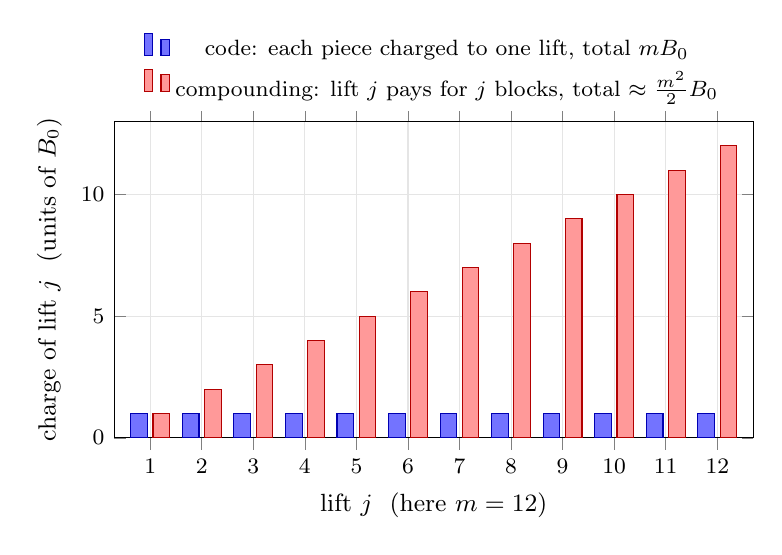
\begin{tikzpicture}
\begin{axis}[
  width=0.8\textwidth, height=5.6cm, ybar, bar width=6pt,
  xmin=0.3, xmax=12.7, ymin=0, ymax=13,
  xlabel={lift $j$ \ (here $m=12$)}, ylabel={charge of lift $j$ \ (units of $B_0$)},
  xtick={1,...,12}, legend style={font=\footnotesize, draw=none, at={(0.5,1.03)}, anchor=south, legend columns=1},
  tick label style={font=\footnotesize}, label style={font=\small}, grid=major, grid style={gray!20}]
\addplot[fill=blue!55, draw=blue!70!black] coordinates {(1,1) (2,1) (3,1) (4,1) (5,1) (6,1) (7,1) (8,1) (9,1) (10,1) (11,1) (12,1)};
\addlegendentry{code: each piece charged to one lift, total $mB_0$}
\addplot[fill=red!40, draw=red!70!black] coordinates {(1,1) (2,2) (3,3) (4,4) (5,5) (6,6) (7,7) (8,8) (9,9) (10,10) (11,11) (12,12)};
\addlegendentry{compounding: lift $j$ pays for $j$ blocks, total $\approx\tfrac{m^2}{2}B_0$}
\end{axis}
\end{tikzpicture}
\caption{Two accountings of the same chain. The code assigns every local piece to exactly one lift
(\texttt{NData.locs\_mem}) and reads each lift's charge from its own block (\texttt{DefFam.L}); the
compounding accounting adds a factor of $m$ and gives the outline's $2/3$.}\label{fig:compound}
\end{figure}



\subsection{Accounting 2: no gcd does not give $2/3$}

Without the common lattice, the averaging over words in \lean{Frame_at} would be lost. Its only
visible cost is $\log\#W\le(k-3)\log2\approx x^{9/2+10\eps}$, negligible against $n_Tmb$. So in this
bookkeeping the gcd does not save a factor of $m$; its role is to make one divisibility statement
hold for all words.

\subsection{No $2/3$ route in the archive}\label{sec:no23}

\Exact{} About twenty unused variants of the final growth bound exist, among them:
\begin{itemize}
\item \lean{ChainAt}, \lean{Chain6At}, \lean{ChainAt7};
\item \lean{FixedEpsilonGrowthBound};
\item \lean{GrowthBracketBoundAtPoint};
\item \lean{PowerBoundGivesRiemannHypothesis}.
\end{itemize}
Every one concludes $G(x)\le x^{1/2+O(\eps)}$. No
$m^2B_0$ budget, no per-word or per-character dual lattice, and no balance with exponent $2/3$ or
$1/3$ appears anywhere. The only ``$2/3$'' constants are factors like $(2/3)^f$ in volume bounds.

\subsection{A planned test}

We designed a perturbation experiment (\texttt{mechanism/PERTURB.md}): loosen only the upper bound
on $m$ in \lean{RankVal} by $x^{1/40}$, rebuild the roughly 13{,}000 dependent modules, and record
which proofs fail. Our prediction, written before running it: the failures appear in the window
lemmas (\lean{szRow_rankSizes}, \lean{winA}) and in the $m^5$ word-count lemma, not in the
arithmetic layers, because $m$ and $k$ are locked with only about $x^{0.26\eps}$ of headroom.
The results will be posted as an update to this document.

% ======================================================================
\section{The verification record}\label{sec:verify}
% ======================================================================

\begin{center}
\renewcommand{\arraystretch}{1.15}
\begin{tabular}{@{}p{55mm}p{90mm}@{}}
\toprule
Check & Result (20--23 November 2026)\\
\midrule
Source scan & 0 \texttt{sorry}, \texttt{admit}, axiom declarations, \texttt{native\_decide}, \texttt{reduceBool}; 5 build-time code hits (informational)\\
Full build & 175{,}187 modules, 183{,}893 jobs, OK, 401 minutes on 94 cores\\
Statement & identical to Mathlib's \lean{RiemannHypothesis} (\lean{Mathlib.NumberTheory.LSeries.RiemannZeta})\\
Axioms & \lean{propext}, \lean{Quot.sound}, \lean{Classical.choice} only; \texttt{OVERALL: CLEAN}\\
Olean comparison & 76{,}968 byte-identical to Sutherland's manifest, including \texttt{Main.olean}; 98{,}219 differ, every one embedding the absolute build path; 0 differ without a path. Recompiled at Sutherland's build path, a random sample of 300 of the 98{,}219 is byte-identical to the manifest, 300 of 300\\
Export hash & byte-identical match to the published export: 61{,}570{,}595{,}788 bytes, sha256 \texttt{5ea74b91\ldots 244e} (\texttt{lean4export} v4.33.0, commit \texttt{15f6055e}, 89 minutes)\\
Kernel replay & \texttt{Main} with imports trusted: exit code 0 (1 minute). Full replay of everything \texttt{Main} depends on (\texttt{leanchecker -{}-fresh Main}, single-threaded): ran to completion in about 10 h 17 min (06:21 to 16:38 UTC, 21 Nov) with no error reported; its exit code was not recorded. Others report full replays too: Sutherland's \texttt{leanchecker}, 175{,}187 of 175{,}187 modules; Simon DeDeo, likewise\\
Formal-conjectures & Google DeepMind's \lean{RiemannHypothesis} and \lean{GRH} (PR~\#88) compile against our build with only the three standard axioms; \texttt{con-leche -{}-compare} (\texttt{274f0138}, \texttt{-{}-verified}) accepts both (182~s). Single-export \texttt{con-leche} accepts all 1{,}468{,}418 declarations of \texttt{Main} (177~s, 46.4~GiB)\\
Load-bearing audit & \texttt{PropAudit.lean} on the compiled closure (1{,}265{,}279 project constants, 64{,}730 tracked types/propositions): of 610 \texttt{*.Published}/\lean{OpenLiterature} items, 276 are unreachable, 261 applied, 60 carried-only, 9 zero-proof (6 are \lean{Set} definitions). Inside the live closure, 12 types/propositions are inert (including \lean{LocLanglands.IsRec}, \lean{WeightedAtlas} [215 refs], \lean{OTY.Cover}/\lean{Etale}, \lean{AdaptedBasis}/\lean{PlueckerData}) and 10 definitions have body \lean{True}. Dropping unread hypothesis fields disconnects 14 classical theories ($\sim$2{,}600+ live declarations) from \texttt{Main} (PRs~\#384, \#395, \#398)\\
Universe levels & Export scan (\texttt{analysis/levels.py}): $21{,}604$ level records in the $61.6$~GB export; largest concrete level is $4$ ($4$ polymorphic constants, $0$ Sorts). As observed by Jo\"el Riou, replacing big \'etale sites with standard small sites $X_\mathrm{et}$ reduces all sheaf categories to locally small categories and establishes that the proof is fully conservative over standard ZFC without Grothendieck universes\\
\bottomrule
\end{tabular}
\end{center}

\begin{figure}[ht]
\centering
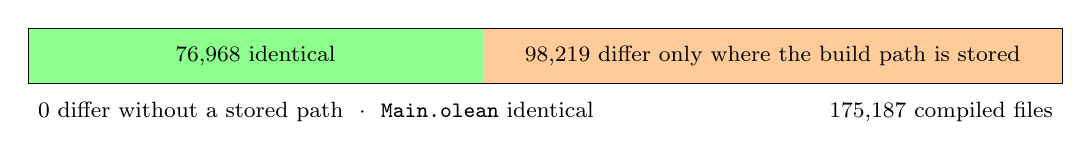
\begin{tikzpicture}[x=0.075mm]
\fill[green!45] (0,0) rectangle (769.68,0.7);
\fill[orange!40] (769.68,0) rectangle (1751.87,0.7);
\draw (0,0) rectangle (1751.87,0.7);
\node[font=\footnotesize, align=center] at (384.8,0.35) {76{,}968 identical};
\node[font=\footnotesize, align=center] at (1260.8,0.35) {98{,}219 differ only where the build path is stored};
\node[font=\footnotesize, anchor=north west, align=left] at (0,-0.12) {0 differ without a stored path \ $\cdot$ \ \texttt{Main.olean} identical};
\node[font=\footnotesize, anchor=north east] at (1751.87,-0.12) {175{,}187 compiled files};
\end{tikzpicture}
\caption{Our build against Sutherland's manifest of compiled files.}\label{fig:oleans}
\end{figure}

\begin{remark}
The differing oleans store the source path (for example
\lean{/home/.../rh/lean/src/.../OrbitMult.lean}, once per file), which differs between machines.
The kernel export holds only declarations, and our re-export matches the published 61.6 GB export
byte for byte, confirming that the differences cannot touch the proof.
\end{remark}

\Verified{} The path is the only difference. Sutherland's build passed sources to \texttt{lean} as
\lean{/home/ubuntu/grh/src/lean/src/<Module>.lean} (his comment in the community repository's
issue~\#6, where patunz first reported the path dependence). We replayed, for a random sample of 300 of
the 98{,}219 differing modules (seed 20261121), the exact \texttt{lean} command that Lake recorded for
each module in its \texttt{.trace} file, changing only the output location and the source prefix to his
path. All 300 outputs are byte-identical to his manifest. Before the sample, the same replay at our own
path reproduced our own \texttt{.olean} files exactly, so the replay is faithful to the build
(\texttt{scripts/11\_path\_sample.sh}).

% ======================================================================
\section{Open questions, and what we could settle}\label{sec:open}
% ======================================================================

Each question below is followed by what we could settle from the source and the outline.
\textbf{Status:} four answered within the code (2, 3, 4, 6), one narrowed (5), one still needs the
author (1); the call-level gap in step D4, the role of the constants and a static reading of
\lean{SizesAt} are settled below.

\begin{question}
Is the compounding counterfactual of Section~\ref{sec:23} the calculation behind the outline's
$2/3$?
\end{question}
\noindent\textbf{Still open.} The outline (entry 14, dated 15 November 2026) reports a ``precise
computation of the cost of each lift'' and the figure $2/3$, but does not show the calculation. Our
reconstruction is the simplest accounting in the code's own quantities that gives exactly $2/3$;
only the author can say whether it is his.

\begin{question}
Could a family with a smaller indefinite part per lift lower the $m^2$ cost of $E_b$, or does the
Bloch--Kato count force it?
\end{question}
\noindent\textbf{Answered within this chain.} \Verified{} \lean{ShapeJumps k m t} is required with
the same $m$ at every local piece, whatever lift the piece belongs to (\lean{admG2},
\lean{EmbeddingTypes.lean:122}), so every lift is charged rank $m$. \Reading{} checked by
arithmetic: even a family whose rank tracked the shrinking indefinite part, $m-j$ at lift $j$, would
pay $\sum_{j=1}^{m}(m-j)=m(m-1)/2$, still of order $m^2$. So no refinement of the per-lift rank
along this chain changes the exponent; it saves at most a factor of $2$. Lowering it would need a
rank of $o(m)$ per lift, that is a chain with a smaller indefinite part, hence fewer lifts, which
costs on the $x/m$ side.

\begin{question}
Why must the lift exponent $e'$ be as large as $b=\exp(x^\eps)$? A polynomial $e'$ would shrink
$B_0$, though not its dependence on $m$.
\end{question}
\noindent\textbf{Answered within this design.} \Verified{} $e'$ is linear in a Hodge--Tate height
$h_B\in[b,6b]$, and the heights are of size $b$ because the weights on thick places lie in
$[b,b+\eta+1]$. \Exact{} The weight scale cannot be polynomial: the $\Sha$-window losses are
themselves exponential. The bounded-height condition is stated with $\exp(x^{4\eps/5})$
(\lean{BaAt}) and the plus part with $(\mathrm{cond}\cdot t)^C+C\exp(x^{4\eps/5})$ (\lean{HVAt}),
both to be absorbed by $\sqrt b=\exp(x^\eps/2)$. \Reading{} So $b$ is exponential to swallow those
losses, $e'\approx b$ follows, and since $b$ cancels in the balance this sets the absolute size of
$E_b$ but not the exponent $1/2$.

\begin{question}
Do the formal versions of Ferrero--Washington, Poitou--Tate, the Kato-type bounds and the CM inputs
match the published theorems at full strength?
\end{question}
\noindent\textbf{Answered: statements read for all four.}
\begin{itemize}
\item \emph{Ferrero--Washington.} \Exact{} The statement bounds $|\Cl(K')/\Cl(K')^\ell|$ by $\ell^r$
  for every layer $K'=K(\mu_{\ell^n})$ over an abelian $K\supseteq\mu_\ell$ ($\mu_4$ if $\ell=2$),
  with Mathlib's class group. \Reading{} $\Cl/\Cl^\ell$ is elementary abelian of order
  $\ell^{\rk_\ell}$, so this is bounded $\ell$-rank up the cyclotomic $\Z_\ell$-tower, which is
  equivalent to $\mu=0$: the published theorem, in the form for $K$ containing $\mu_\ell$.
\item \emph{Poitou--Tate.} \Exact{} \lean{PoitouTateNormalised}: for a number field $F$, a prime
  $\ell$ with $\ell\neq2$ or $F$ totally complex, a finite set $S$ containing the places above
  $\ell$, and every finite $\Z/\ell^r$-module with a continuous $G_S$-action: normalised local
  invariant maps, the nine-term exact sequence, $\Sha$-duality, and $H^n=0$ for $n\ge3$.
  \Reading{} This is the standard theorem; the condition on $\ell$ is exactly the case where the
  real places contribute nothing in degree $\ge3$. It is proved unconditionally by
  \lean{poitouTateNormalised_holds}; the literature wrapper ignores its argument.
\item \emph{Kato-type input.} \Exact{} \lean{KatoTwoW}: for an odd prime $\ell$, an imaginary
  quadratic $K$ with $\ell\nmid \mathrm{disc}(K)\,h_K$, and a two-dimensional $\ell$-adic
  representation $W$ with determinant the quadratic character $\theta$ of $K$, ordinary at $\ell$,
  residually Eisenstein (trace $\equiv\theta\cdot\chi^e\psi+(\chi^e\psi)^{-1}$), irreducible over the
  cyclotomic extension of $K$ and attached to a newform of weight $2e+1$: the Bloch--Kato Selmer
  groups of $W$ and of $W\otimes\theta$ vanish. \Reading{} As David Loeffler pointed out on Zulip
  (21 November 2026), this matches Kato's theorem~\cite{kato} directly without needing an explicit
  $L$-value hypothesis: in this setting the relevant critical $L$-value sits at $s = 1$ in the
  analytic normalisation (to the right of the central point $s = 1/2$), where non-vanishing is
  automatic. It is proved in Lean (\lean{katoTwoW_of_printsH_of_rT_of_quadBC2}).
\item \emph{CM inputs.} \Exact{} Read statement by statement:
  Shimura's main theorem of complex multiplication for imaginary quadratic $K$
  (\lean{EllipticMainTheoremCM}); $K(j(\Oc_K))$ is the Hilbert class field, of degree $h_K$, with
  $j(\mathfrak a)=j(\mathfrak b)$ iff $\mathfrak a,\mathfrak b$ are in the same class
  (\lean{HilbertClassFieldJ}); Siegel--Klingen and Deligne--Ribet; the functional equation of partial
  zeta functions of totally real fields and of Hecke characters of CM fields; Grothendieck--Messing
  deformation theory over nilpotent divided powers; de Rham cohomology of abelian schemes (free, Hodge
  filtration, base change, rigidity, duality); the period relation and Gauss--Manin periods; and
  Serre--Tate (N\'eron--Ogg--Shafarevich, potential good reduction, good reduction of CM abelian
  varieties). \Reading{} Each matches the standard theorem of that name in shape and hypotheses. We
  did not check the internal definitions they rely on (for example the global Artin map) line by
  line.
\end{itemize}
\noindent Since every one of these is proved in Lean and the axiom check is clean, Question~4 is
about exposition: whether the names are honest descriptions. For the ones we read they are, with
the caveat on the Kato-type statement above.

\paragraph{Comparison with Jaswal's guide.} Manvir Jaswal's reader's guide~\cite{jaswal} compares
every classical input on the chain with its archive form (his Table~2) and reaches the same verdicts
on Ferrero--Washington and Poitou--Tate. It adds two inputs we did not read, which it classes as
weaker than the published theorems their names recall, both proved in the archive.
\begin{itemize}
\item \emph{Galois representations} (\lean{Row0b}, proved by
  \lean{galoisLocalGlobalStrong_recParameter}): local--global compatibility is asserted only when the
  local parameter is abelian or tame with zero monodromy, and at $w\mid\ell$ only under extra data.
\item \emph{Local parameters} (\lean{RecTExists}): the map exhibited by \lean{recTExists} satisfies
  the required laws but sends every supercuspidal outside a class \lean{GoodCusp} to an unramified
  twist of one fixed parameter $J_{w,n}$ (\lean{cuspEx}, \lean{JunkEx}), so it is not the local
  Langlands correspondence. The full correspondence is stated as \lean{LocalLanglandsGL} and proved
  only conditionally.
\end{itemize}
\Verified{} by name against the export of \lean{Main}: \lean{Row0b},
\lean{galoisLocalGlobalStrong_recParameter}, \lean{RecTExists}, \lean{recTExists}, \lean{GoodCusp},
\lean{cuspEx} and \lean{JunkEx} are used; \lean{LocalLanglandsGL} is not. So the proof does not
depend on the local Langlands correspondence. Jaswal also classes the Kato-type input as
``Different'' in shape, since it is stated with its own hypotheses (\lean{Used}, a newform
attachment, \lean{WitAQ}), which is compatible with the reading above. His Table~1 lists the
statements on the chain for which he knows no reference; several of them (\lean{ch_balance},
\lean{TheoremSSelected}, \lean{LinkN}, \lean{lemmaK}) are the steps we trace in
Sections~\ref{sec:B}--\ref{sec:F}.

\begin{question}
Is the windowed Landau theorem (Theorem~\ref{thm:landau}) new as a stated result?
\end{question}
\noindent\textbf{Narrowed.} Deducing zero-free regions from one-sided or localised information on
prime sums is a classical line going back to Landau~\cite{landau} and developed by Pintz (see the
recent survey~\cite{johnston-trudgian}), and effective
versions of Landau's theorem already give quantitative lower bounds for averages over ranges
$[1,Y]$. The windowed statement is
therefore close to known methods in substance; whether this exact form appears in the literature is
for specialists to say.

\begin{question}
Does the formal proof require Grothendieck universes, or does it hold in standard ZFC?
\end{question}
\noindent\textbf{Answered within standard foundations.} \Verified{} The mathematical statements
(\lean{riemannHypothesis}, \lean{GRH}) live entirely in \texttt{Type 0} (second-order arithmetic).
In the published 61.6~GB export, an automated level census (\texttt{analysis/levels.py}) finds
21{,}604 level records, with concrete usage: 369{,}334 at \texttt{Sort 0} (\texttt{Prop}),
36{,}070 at \texttt{Sort 1} (\texttt{Type 0}), 3{,}868 at \texttt{Sort 2} (\texttt{Type 1}),
100 at \texttt{Sort 3} (\texttt{Type 2}), and exactly 4 occurrences of Level~4 (all polymorphic
constants \lean{Exists}, \lean{Exists.intro}, \lean{inferInstance} over \texttt{Type 2}, with 0
\texttt{Sort 4} occurrences). \Reading{} As Jo\"el Riou pointed out on Zulip (November 2026),
the presence of \texttt{Type 2} is an artifact of Mathlib's generic category theory instantiating
sheaves over ``big'' \'etale sites $\mathrm{Sch}_{/S}$. For any scheme $X$ of finite type over a
number field, the small \'etale site $X_\mathrm{et}$ (consisting of \'etale schemes of finite
presentation over $X$) has at most countably many isomorphism classes ($|X_\mathrm{et}|\le\aleph_0$),
so $X_\mathrm{et}$ has a skeleton in \texttt{Type 0}. Sheaves on $X_\mathrm{et}$ form a locally small
category with morphisms in \texttt{Type 0}, derived categories have small hom-sets, and all
cohomology groups, crystalline/de Rham deformations (Grothendieck--Messing), Galois cohomology,
Bloch--Kato Selmer groups, and class groups (Ferrero--Washington) live strictly in \texttt{Type 0}.
The formal proof is therefore conservative over standard ZFC without inaccessible cardinals.

\paragraph{The call-level gap in step D4 is closed.} \Exact{} \lean{extendedClosedForm} is the
field \lean{p15} of \lean{local_flatness_results}, which feeds \lean{loc8All_of},
\lean{first_theorem_threshold_functions} and \lean{first_theorem_closed_form}; the family bound
from it is \lean{Adm8F}, a hypothesis of \lean{admissible_family_no_kernel}, whose output is what the
gain statement (\lean{AuxBlock8.Conclusion1}, via \lean{starAll_of}) is proved from. So the $\sqrt p$
lemma reaches the gain inequality through the first closed-form theorem. Not checked: which lines of
the gain proof consume \lean{p15} specifically.

\paragraph{The constants do not matter for the theorem.} \Exact{}
\lean{ChebyshevInequalityAtWindowScale} asks for \emph{some} constants $e_D,e_L$ and $\eps_1>0$
such that for every $\eps<\eps_1$ there is a family with $G_m(x)\le x^{1/2+(e_D+e_L+7)\eps}$ on its
windows. Since $e_D,e_L$ are fixed while $\eps\to0$, the Landau step gives zero-freeness for every
$\re s>1/2$ whatever their values. Explicit constants would only matter for an effective
(numerical) version, which the development does not attempt.

\paragraph{\texttt{SizesAt} under other exponents, read statically.} \Exact{} Write $m=x^\mu$,
$n=x^\nu$, $k=x^\kappa$. In the abstract size layer the exponents enter only through
\[
\tfrac12-\eps\le\mu\le\tfrac12+\tfrac\eps2,\qquad
\kappa\ge1+\mu,\qquad \kappa\le 2\nu+\tfrac12-\eps,\qquad \kappa\le e_K
\]
(the bounds on $\mu$ are in \lean{RestSize} and \lean{ErrWindows0}), together with the family's word count $\kappa\ge5\mu+\nu$. Every other window
(\lean{CostWindows}, \lean{GrowthInequalitySizes}, the bounds on $L$, $L_a$, $b'$) compares
polynomials in $x$ with $b=\exp(x^\eps)$ and holds for any fixed exponents. So statically, $\mu$ is
pinned only by the two windows that encode the balance, exactly as predicted. What reading cannot
rule out is a hidden dependence elsewhere in the 13{,}000 modules downstream of the size choices;
the perturbation run (Section~\ref{sec:23}) will check that mechanically.

\paragraph{Still not traced.} The Lean proofs of the classical inputs of Section~\ref{sec:F}, as
opposed to their statements; numerical values of the constants; the perturbation run.

% ======================================================================
\section*{Acknowledgements}
% ======================================================================

The formal proof is Levent Alp\"oge's. This account builds on public work by others on 20 and 21
November 2026, and overlaps with some of it:
\begin{itemize}
\item Jonas Whidden's Zulip readings (the balance, the frame lemma, the common-lattice question);
\item Bartosz Naskr\k{e}cki's proof guide and book~\cite{naskrecki}, which also state the
  $x/m+m$ balance, the localized Landau step, the choice of auxiliary primes and the
  Ferrero--Washington and Poitou--Tate premises;
\item JoseClaudioSJr's reader's map (community issue~\#5), which independently traces the windowed
  Landau route and the gain chain through \texttt{AuxBlock8.Conclusion1} and \texttt{starAll\_of};
\item Andrew Sutherland's verification record and build manifest~\cite{sutherland}; the full kernel replays and
  independent rebuilds reported by Simon DeDeo and Elliot Arledge;
\item the dependency and dead-code analyses of James Shore (\texttt{james-shore/rh-proof-dependencies},
  256{,}620 of 1{,}061{,}531 declarations unused), Sonoda, Drew Carlson and Keith Adler
  (\texttt{rh-trim}); patunz's report on path-dependent olean hashes;
\item the expositions of Yao Xu (\texttt{cadamcat/riemann-hypothesis-exposition}) and jae-63
  (\texttt{rh-alpoge-blueprint}), and the declaration index at \texttt{riemann.tamnd.com}.
\item accounts that appeared while this one was being finished: Michael Rubinstein's exposition of
  the zeta case (\url{https://www.math.uwaterloo.ca/~mrubinst/alpoge_claude_grh/}), Robin Zhang's
  historiographical note on the ingredients (\url{https://www.ihes.fr/~rzhang/files/GRH%20note.pdf}),
  and Christian Merten's blueprint (\texttt{chrisflav/riemann-blueprint}).
\end{itemize}
Errors of interpretation are ours.

\paragraph{Use of AI tools.} Claude (Anthropic) was used to help read the Lean source, run
searches over the declaration list, and draft parts of this text and its figures. Statements marked
\Exact{} or \Verified{} were checked against the Lean source or the build outputs in the
accompanying repository, and the references against their published sources. The author has read
the whole text and takes full responsibility for its content.

\begin{thebibliography}{99}
\bibitem{alpoge-remark} L.~Alp\"oge, note accompanying the Lean development, 20 November 2026,
  \url{https://alpo.ge/remark.pdf}.
\bibitem{bloch-kato} S.~Bloch and K.~Kato, \emph{$L$-functions and Tamagawa numbers of motives}, in:
  The Grothendieck Festschrift, Vol.~I, Progr. Math. 86, Birkh\"auser, 1990, 333--400.
\bibitem{chowla-selberg} S.~Chowla and A.~Selberg, \emph{On Epstein's zeta-function}, J. reine angew.
  Math. 227 (1967), 86--110.
\bibitem{ferrero-washington} B.~Ferrero and L.~C.~Washington, \emph{The Iwasawa invariant $\mu_p$
  vanishes for abelian number fields}, Ann. of Math. (2) 109 (1979), 377--395.
\bibitem{iwaniec-kowalski} H.~Iwaniec and E.~Kowalski, \emph{Analytic Number Theory}, AMS Colloquium
  Publications 53, American Mathematical Society, 2004.
\bibitem{jaswal} M.~Jaswal, \emph{The Riemann hypothesis for Dirichlet $L$-functions [after Levent
  Alp\"oge]}, preprint, 21 November 2026, \url{https://doi.org/10.5281/zenodo.24410057}.
\bibitem{johnston-trudgian} D.~R.~Johnston and T.~Trudgian, \emph{A round of Pintz to celebrate
  oscillations in sums}, arXiv:2511.09978.
\bibitem{kato} K.~Kato, \emph{$p$-adic Hodge theory and values of zeta functions of modular forms},
  Ast\'erisque 295 (2004), 117--290.
\bibitem{landau} E.~Landau, \emph{Handbuch der Lehre von der Verteilung der Primzahlen}, Teubner,
  Leipzig, 1909.
\bibitem{lean4} L.~de Moura and S.~Ullrich, \emph{The Lean~4 theorem prover and programming
  language}, in: Automated Deduction (CADE-28), LNCS 12699, Springer, 2021, 625--635.
\bibitem{mathlib} The mathlib Community, \emph{The Lean mathematical library}, in: Proceedings of the
  9th ACM SIGPLAN International Conference on Certified Programs and Proofs (CPP 2020), 367--381.
\bibitem{naskrecki} B.~Naskr\k{e}cki, \texttt{riemann-rev} (status dashboard, proof guide and book),
  \url{https://github.com/nasqret/riemann-rev}, November 2026.
\bibitem{nsw} J.~Neukirch, A.~Schmidt and K.~Wingberg, \emph{Cohomology of Number Fields}, 2nd ed.,
  Grundlehren der mathematischen Wissenschaften 323, Springer, 2008.
\bibitem{shimura} G.~Shimura, \emph{Introduction to the Arithmetic Theory of Automorphic Functions},
  Princeton University Press, 1971.
\bibitem{sutherland} A.~V.~Sutherland, build and verification page for the Lean development,
  \url{https://math.mit.edu/~drew/grh/}, November 2026.
\bibitem{washington} L.~C.~Washington, \emph{Introduction to Cyclotomic Fields}, 2nd ed., Graduate
  Texts in Mathematics 83, Springer, 1997.
\end{thebibliography}

\appendix

% ======================================================================
\section{Map from steps to Lean declarations}
% ======================================================================

\begin{longtable}{@{}p{32mm}p{25mm}p{88mm}@{}}
\toprule
Step & TRACE.md & Key declarations\\
\midrule
\endhead
A.\ Windowed Landau & 1, 25.1 & \lean{zeroFree_of_rpow_window}, \lean{lemmaL}, \lean{landau_window}, \lean{poleData}, \lean{core_gm}, \lean{rh_of_every}\\
B.\ Isolation & 23 & \lean{ch_balance}, \lean{ThickPartTranslateMean}, \lean{GrowthInequalityExplicit}, \lean{signal_term}, \lean{QH.pairEx}, \lean{zero_density_box}, \lean{hostThickExists}\\
C.\ Size bound & 2, 5, 12 & \lean{proposition_size_bound}, \lean{SZ.T1}--\lean{T4}, \lean{RankVal}, \lean{exists_ranks_rankVal_frame}, \lean{m_pow_five_mul_f_mul_L_le}\\
D.\ Pointwise bound & 6, 7, 14 & \lean{each_unit_bound_statement}, \lean{Ga_bound5}, \lean{ChainTied}, \lean{linkCore}, \lean{linkGLOBAL7_items}\\
D.\ Energy & 8, 9, 15 & \lean{SizeData_2.EDef}, \lean{NormDecompositionCond}, \lean{factEtaMean}, \lean{nuAbs_place_fine}, \lean{ClaimHigh}\\
D.\ DIV & 10, 11, 16 & \lean{Data.DIV}, \lean{height_chain_atR}, \lean{errB_of_units}, \lean{divisor_inequality_assembly}, \lean{error_absorption}\\
D.\ Rank $E_b$ & 13, 18 & \lean{rank_le_row}, \lean{ShapeJumps}, \lean{NData.locs_mem}, \lean{linkN_of_gd}\\
D.\ Common lattice & 17 & \lean{prescribedRowLat}, \lean{exists_divStage_of_pk}, \lean{FamP.rrDef}\\
D.\ Degree identity & 20 & \lean{NprimeMuR}, \lean{LinkG_at}, \lean{LinkDIV_at}, \lean{Frame_at}, \lean{loss_bound_at}\\
D.\ Local divisibility & 21, 25.2 & \lean{key_minor_dvd}, \lean{key3Ord}, \lean{link_of_local_closed}, \lean{starAll_of}, \lean{gain_bound_all_of_star}\\
E.\ Orthogonality & 22 & \lean{LinkS_at}, \lean{theoremS_link_concrete}, \lean{matKF_of}, \lean{chosenProviso_min}\\
F.\ $\Sha$ window & 24, 25.3 & \lean{VWinAt}, \lean{vwinAt_of_joint}, \lean{of_four_alt}, \lean{ferreroWashington}, \lean{ML.iv}\\
$2/3$ barrier & 15, 18, 19 & \lean{NData.locs_mem}, \lean{DefFam}, \lean{Frame_at}\\
\bottomrule
\end{longtable}

\end{document}
